\chapter{Introduction}
Technology is evolving faster every year which also applies to biometric systems. Fingerprint-based biometric systems are faster than ever gaining acceptance to be used as one of the most effective technology for authentication. Nowadays we use fingerprint-based biometric features not only to unlock our smartphones but even to log into our bank accounts or as a proof of identity on borders in some countries. But as always in technology, when something moves forward the attackers do as well. And in the case of bank accounts or proof of identity, nobody wants to be cracked.

There is put much of afford and work into making sensors and the whole process more robust. In the case of sensors liveness detection can be used as an example, but this feature as many others can not be used in every situation mostly because of its size as an example can be used in smartphones. And the second part that is instantly improving is the algorithm itself. For improving the algorithm there is a lot of testing needed, which brings one big problem and it is a big database of fingerprints. Database means not only a lot of fingerprints from one finger under different angles but also a lot of fingerprints from different people. Therefore there are a lot of algorithms for generating fingerprints used just to make larger databases more than for attack systems.

This work is mainly focused on known fingerprint generation by morphing. This field of generation was not researched much yet, where basically only one paper from the year 2017 was made public and it includes a lot of uncertainties. This work is trying to describe these uncertainties and find improvements in the process of already described morphing and also test the solution against the used biometric systems.

Chapter two describes the theory that is needed to be known before getting familiar with the algorithm itself and trying to get its principle. Not only theory needed for implementation is included in this chapter, but also the basics about fingerprints and capturing fingerprints with sensors. The third chapter describes the proposal of all stages of an improved algorithm from the paper mentioned before. The fourth chapter describes an implementation of morphing application and also the second part of this work which is an implementation of fingerprint matching scripts with the use of tools from companies Innovatrics and Neurotec. Where in the fifth chapter are the results of these two scripts compared against implemented algorithm with the use of a database borrowed from the FIT by a supervisor of this work. 

\chapter{Biometrics} \label{theory}
There is described all the theory needed to understand the solution of this thesis in this chapter. This thesis deals with fingerprint generation as it is obvious from the name but the thesis includes the comparison of results against real working solutions as well. The comparison includes an understanding of fingerprint recognition techniques. Both problems fall into the field of biometrics. 

\section{Introduction to biometrics}
It is necessary to explain from the beginning, what to imagine under the word biometrics in the field of information technology. The term biometrics in our context means the automatic recognition of a person on the basis of their characteristic physiological and behavioral properties. Three basic methods are defined for recognizing people: a) what a person knows b) what a person has c) what a person is (biometrics, for example, just a fingerprint). While recognition methods based on knowledge (eg password) or ownership (eg key) can be forgotten/lost, guessed/stolen, or shared in some way. \cite{jain2011introduction} Since we still have the biometric properties of our body with us, they are mostly not possible to lose and not to be forgotten at all. However, this is also the biggest weakness of biometric systems, which basically means once some biometric feature is discovered, we no longer have the opportunity to change it.\cite{maltoni2009handbook}

There are many important terms in the field of biometrics. Interclass and intraclass variability are among them. Interclass variability says how big is the difference between individual classes (in our case the class is people and we want this feature to be as different as it can be). On the opposite hand, there is the intraclass variability, which sets the differences between the same class (in our the same person). There are seven basic features for comparison of biometrics characteristics\cite{maltoni2009handbook}:

\begin{itemize}
    \setlength\itemsep{0.2em}
    \item Universality = Each person should have this feature
    \item Uniqueness = The feature should differ for each person
    \item Permanence = The feature should stay the same over the time 
    \item Measurability = Biometrics is easily acquired
    \item Performance = Recognition accuracy, speed, resource requirements, etc.
    \item Acceptability = Willingness to capture the feature 
    \item Circumvention = Difficulty to create working fake feature \cite{maltoni2009handbook} \cite{jain2007handbook} \cite{01BioPrednaska}
\end{itemize}

There is no expectation at all that any biometrics will be perfect in all these characteristics. This means that no biometrics is ideal, but most of them are acceptable. When choosing which biometrics to use, the decision needs to be made based on the requirements of an application and the features of that biometrics.

\section{Fingerprint}
The fingerprint is made by the representation of the epidermis, where the pattern is made by interleaving ridges and valleys. The epidermis itself is in the highest level creating skin together with dermis (called real skin) and subcutaneous (fat) layer  \cite{jain2007handbook}(viz. figure \ref{fig:skin}).

\begin{figure}[H]
    \centering
        {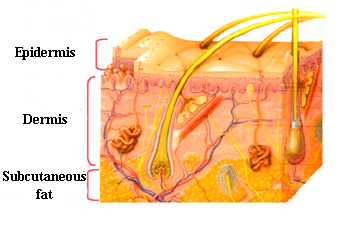
\includegraphics[width=0.6\linewidth]{obrazky-figures/skin.png}}\\
        \caption{Skin structure \cite{Skinanat76:online}}
        \label{fig:skin}
\end{figure}

A combination of genetic and environmental factors is creating the pattern of the ridges in the process of growing capillaries and blood vessels in angiogenesis. Basically, the forming of skin is made by genetic code but the specific way that skin will look like is the result of random acts on the child in his mother’s womb. This is the reason why there is no identical biometrics even in the case of identical twins. The final look of the fingerprint is made approximately in the first seven months of fetal development and then it is the final form. It means that the configuration of papillary lines is not changing throughout a life of a person except for some injuries. And this makes our fingerprints a very attractive biometrics feature for identification. \cite{maltoni2009handbook} \cite{babler1991embryologic}

Typically the fingerprints are taken in the form that the ridges are dark lines and on the other hand the valleys are light (figure 2.3). Ridges are usually from 100 µm to 300 µm wide and the valleys are around 500 µm wide. The injuries are usually only small scratches or so, and these small injuries usually do not go to the underlying structure of the ridge so the pattern stays unchanged after regeneration. \cite{maltoni2009handbook}

\begin{figure}[H]
    \centering
        {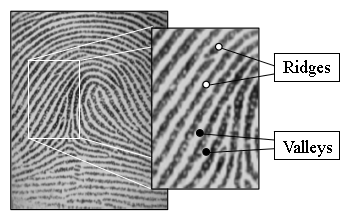
\includegraphics[width=0.5\linewidth]{obrazky-figures/print.png}}\\
        \caption{Fingerprint \cite{maltoni2009handbook}}
        \label{fig:fingerprint_1}
\end{figure}

\subsection{Improvements of fingerprint image and binarization}
The quality of input images plays a big role in algorithms that implements minutiae extraction and fingerprint recognition. Actually, in real applications even bad conditions like too wet/dry skin, small injuries, bruises, bad pressure on the fingerprint sensor or bad fingerprints (older people or hand working people) is a high chance (around 10$\%$) that the fingerprint is no acceptable.\cite{jain2007handbook}

Therefore is the algorithm for improving fingerprints images. It improves brightness, the clarity of ridges in places where it is still possible, and marking places where it is not possible as too noisy for next processing. The most common way how to do the improvement is based on context filters. Characteristics of the filter are changing based on the local neighborhood in the context filtering. The change is mostly based on local ridge orientation and local ridge frequency. The unwanted noise and preservation of the true structure of the ridge and valley can be achieved by choosing the right filter.\cite{jain2007handbook} 

\begin{figure}[H]
    \centering
        {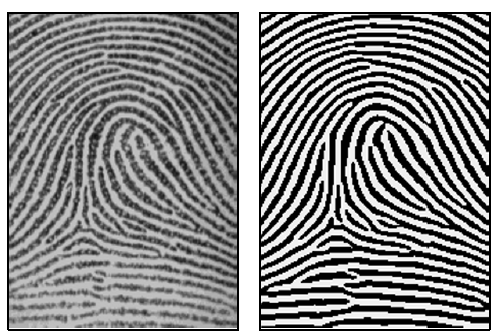
\includegraphics[width=0.6\linewidth]{obrazky-figures/enhancement.png}}\\
        \caption{There can be seen result after binarisation in the right picture as a result coming from left picture. \cite{maltoni2009handbook}}
\end{figure}

\subsection{Fingerprint analysis}
Ridges contain a lot of information and there are three basic levels that describe the amount of extracted information. The first level extracts only the global pattern of ridge flow. The second contains information about minutiae and the third is the most complex and includes information about pores, the local shape of ridge edge, and even more. \cite{jain2007handbook} \cite{maltoni2009handbook}

When we look at ridges globally (1st level), they usually run smoothly and parallel but there can be found at least one area, where some changes can be found like high curvature of ridges or frequent ridge endings. We call these areas singularities or singular areas and they can be divided into three topologies which are \emph{whorl}, \emph{delta}, \emph{loop}. Areas that contain these three topologies are usually marked with these shapes:  $\cap$, $\Delta$ a O. \cite{jain2007handbook} \cite{maltoni2009handbook}

The alignment of fingerprints can be done in some applications by aligning two fingerprints \emph{core} on the core. The core of fingerprint was defined by Edward Henry as "The northernmost point of the innermost ridgeline". In the end, everything depends on what is used in the applications and it is the point of the center of the singularity of the northernmost loop type. (eg Those that belong to the arch class in the figure \ref{fig:classes}). Sometimes it is hard to detect core because some fingerprints simply do not contain whorl or arch, like those which fit into the class of the arch \ref{fig:classes}. In these cases, the core is identified as a point with maximal curvature of the ridge. Because of the high variability of fingerprints, it is hard to identify the core in all the images of fingerprints. Singular points that are used for classification can be seen in figure \ref{fig:classes} and it is used in the way to fasten the classification by working only over fingers with the same class. \cite{maltoni2009handbook}

\begin{figure}[H]
    \centering
        {\includegraphics[width=0.7\linewidth]{obrazky-figures/závitnice.png}}\\
        \caption{Singularities of fingerprint\cite{maltoni2009handbook}}
        \label{fig:singularities}
\end{figure}

\begin{figure}[H]
    \centering
        {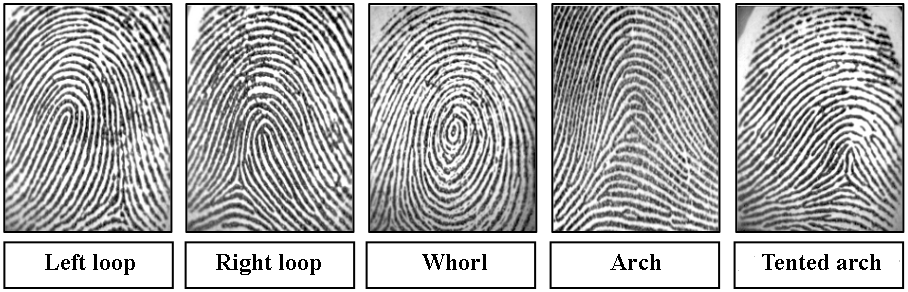
\includegraphics[width=1\linewidth]{obrazky-figures/classes.png}}\\
        \caption{Each fingerprint is representative for each of one of five classes \cite{maltoni2009handbook}\cite{henry1900classification}}
        \label{fig:classes}
\end{figure}

Important points called minutiae can be found in the pattern on a local level (2nd level). Most of the known and used methods for minutia extraction works with binarized images for which the image needs to be transferred to a grayscale image. After the binarization process called thinning is applied which result are ridges of width only 1px. At the end of scanning of the image those pixels which are known as minutiae can be detected. There are many minutiae (some of them can be seen on picture \ref{fig:minutiae}), but most implementations are using just two which are: 1) ridge ending (termination) or ridge division (bifurcation). Most applications use just these two because of the higher accuracy. \cite{jain2007handbook} \cite{maltoni2009handbook}

American National Standards Institute (ANSI) has designed a taxonomy of minutiae based on four classes: termination, bifurcation, trifurcation, and not known. But even the model of the FBI is working only with termination and bifurcation. \cite{maltoni2009handbook}

\begin{figure}[H]
    \centering
        {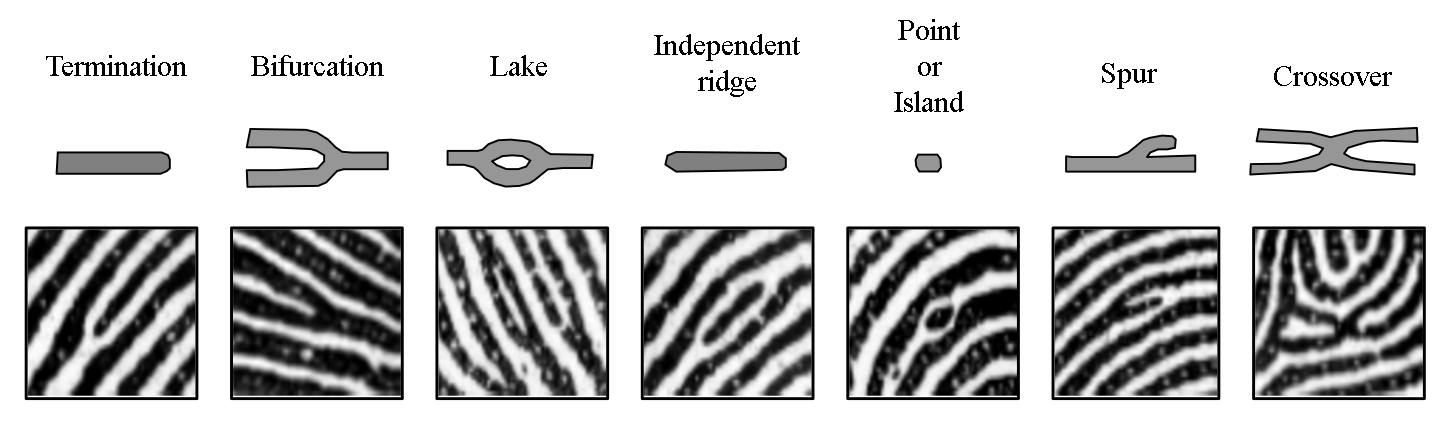
\includegraphics[width=\linewidth]{obrazky-figures/minutiae.png}}\\
        \caption{Seven most common minutiae\ \cite{maltoni2009handbook}}
        \label{fig:minutiae}
\end{figure}

As has been written before there can be taken even more information from the fingerprints for example by pores detection (3rd level). The problem of this level is that pictures of fingerprints need to be taken at very high resolution, which means basically 1000dpi or more. But better results are achieved in the result of using just detection of pores and with a combination of these two methods, significant improvements are done in terms of both. Like I wrote the problem is the high resolution of images, so although achieved improvements this method is not used very often.\cite{jain2007handbook} \cite{maltoni2009handbook}

\subsection{Local ridge orientation}

Local ridge orientation can be counted for every arbitrary neighborhood that some ridge comes through. Then local orientation of the actual ridge at pixel $[x,y]$ is the angle $\theta_{xy}$ in which ridge is coming through the arbitrary big neighborhood with a center in $[x,y]$ arbitrarily forms an angle with the horizontal axis. Because ridges are not coming in specific direction, angle $\theta_{xy}$ is assigned as unoriented direction in $\left[0 ... 180^{\circ}\right]$. Because of the complexity of the computation. Many algorithms work only on discrete positions, which brings even more computing efficiency, and orientation for other pixels is computed by interpolation.

This local ridge orientation is matrix D, which elements are coding local orientation of papillary lines from fingerprints (viz. figure \ref{fig:ori}). Each element $\theta{ij}$  which corresponds to the element $[i,j]$ in a matrix which corresponds to pixel $[x, y]$, then indicates the average orientation of the local neighborhood. Value $r_{ij}$ is often computed for every element $theta_{ij}$. This value $r_{ij}$ stands for reliability or consistency of computed orientation in each block. The high value of $r_{ij}$ means that the picture of the fingerprint is in very good resolution and no big damages are contained in the neighborhood.\cite{maltoni2009handbook}

\begin{figure}[H]
    \centering
        {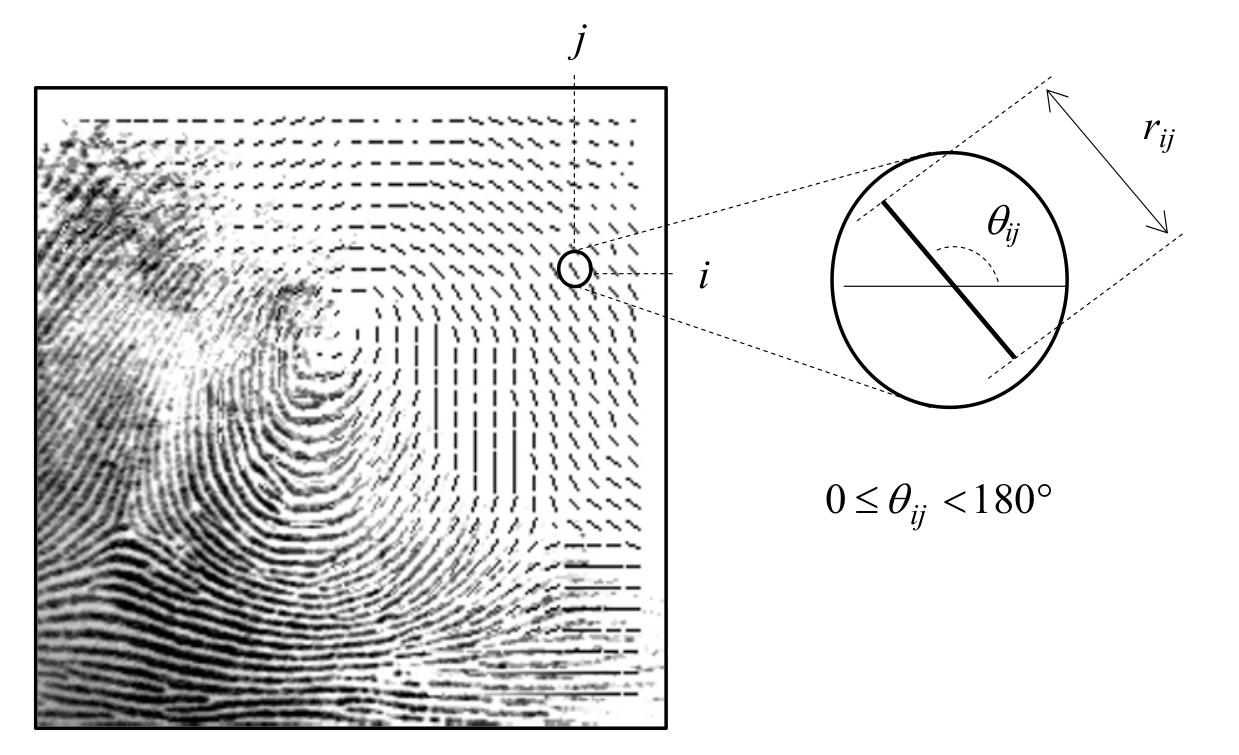
\includegraphics[width=0.6\linewidth]{obrazky-figures/ori.png}}\\
        \caption{The transition of a fingerprint image to the corresponding orientation image is calculated over a 16 × 16 square block grid. Each element indicates the local orientation of the fingerprint papillary lines. \cite{maltoni2009handbook}}
        \label{fig:ori}
\end{figure}

\subsection{Local frequency of ridges}
Local frequency of ridges $f_{xy}$ in pixel $[x,y]$ basically means the count of ridges in some window of given width placed over hypothetic segment with the center in $[x,y]$. Two rules for the window have to be satisfied. The first is that it has to be placed perpendicular to the local orientation of the ridges $\theta{xy}$. And the second is that if the frequency is estimated over discrete positions, the orientation field has to be computed over discrete positions as well. The frequency differs in every fingerprint and can even differ in different areas of the same fingerprint.\cite{maltoni2009handbook}

The local ridges frequency estimation can be computed as the average count of pixels between two consecutive peaks of gray in a grayscale image in the perpendicular direction to the local orientation of papillary line (figure \ref{fig:freq}). For this purpose, the fingerprint is cut by a plane parallel to the $z$ axis and perpendicular to the local ridge orientation.\cite{hong1998fingerprint}

\begin{figure}[H]
    \centering
        {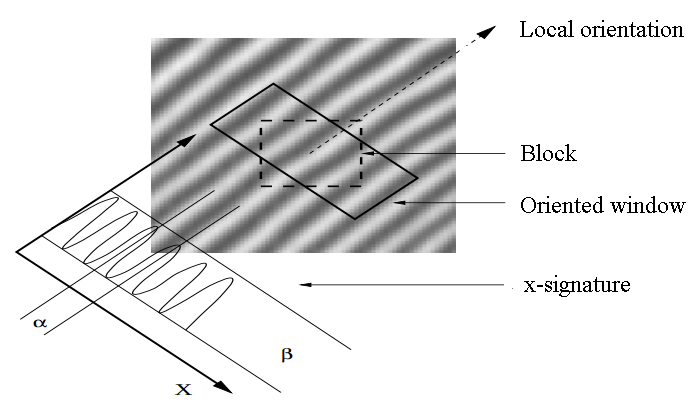
\includegraphics[width=0.7\linewidth]{obrazky-figures/freq.png}}\\
        \caption{Oriented field and x-signature. \cite{hong1998fingerprint}}
        \label{fig:freq}
\end{figure}

\label{sensors}
\section{Fingerprint sensors}
Most AFIS (Automated Fingerprint Identification Systems) for criminal and commercial use are accepting digital images in the input as the result of live scanning acquired by capturing fingerprints by an electronic fingerprint sensor. That means no ink is used and the scanned person has to do only one thing and it is a slight push with his finger to the flat surface of the scanner used for live scanning. The sensor is the most important thing of the whole scanner because it is the part that is creating the fingerprint image. There are three basic types of sensors:\cite{jain2007handbook}   

\begin{enumerate}
	\item \textbf{Optical sensors:} 
	FTIR (Frustrated Total Internal Reflection ) is the oldest and most commonly used technique to capture live scans of fingerprints. The user pushes his finger against the upper side of a scanner, which means that ridges are touching the flat glass surface and valleys are in a short distance. The left side of the prism is illuminated by diffused light. Ridges are absorbing the light coming through the prism to the finger and valleys are reflecting the light. Thanks to this feature it is easy to decide whether it is a ridge or valley. The light rays are coming from the right of the prism and are focused with the lens to CCD or CMOS sensor.\cite{jain2007handbook}     
    
    \item \textbf{Solid-state sensors:}
    Solid-state sensors began to be used commercially in half of the 90s of the last century. Silicon technology for fingerprint live scanning is made from a lot of small pixels and all those pixels are basically small sensors. There is no need for any optical sensor at all, a user just slightly pushes his finger against the surface of the sensor and his fingerprint is scanned. The scanner works on acquiring the physical feature and converts the feature to an electric signal. There are four most used types of silicon sensor: capacitive, piezoelectric, thermal, and electric-field.\cite{jain2007handbook}
    
    \item \textbf{Ultrasound sensors:}
    This last type can be seen also as a type of ultrasound. The sensor operates by sensing the acoustic signal against the finger so by the echo signal the range of depth for fingerprint image can be counted. This method can be useful in places like hospitals or labs because these sensors are scanning subsoil of fingerprint, which means, it can detect the fingerprint over the fluids or even gloves.\cite{jain2007handbook}\cite{maltoni2009handbook}
\end{enumerate}

\subsection{Fingerprint comparison}
One fingerprint can be captured in many different ways, which makes reliable fingerprint comparison a very difficult problem. Movement, rotation, part overlay, nonlinear coloring, variable pressure, skin changes, noise, mistakes in feature extraction all are huge factors that are responsible for intra-class variability. This means that can happen situation where two images of two different fingerprints will have way more in common, than two images of fingerprints of the same person.\cite{jain2007handbook}\cite{maltoni2009handbook}

This is the reason why professional dactyloscopy has to work with many factors before the final verdict if the two fingerprints are from the same person is decided. The factors are: 1. fingerprint has to be from the same class, 2. quantitatively the corresponding features of minutiae must be identical 3. quantitatively a certain number of minutiae must be the same for the examined fingerprints (for example in the USA the minimum is 12 same minutiae) 4. the corresponding features of the compared minutiae must be identical. Special protocols were defined for comparison and there was even created a special diagram to help with dactyloscopy to the detectives if they will ever need to compare fingerprints manually.\cite{maltoni2009handbook}  

The same rules don’t have to be followed in the automatic (commercial) comparison of fingerprints. Actually many new methods were created in the last 50 years which are used only for automation although the basics for detecting minutia and comparison on two fingerprints are based on these rules. It is caused by the need for faster detection but many times at the price of worse results. There are three main ways how to compare fingerprints: \cite{jain2007handbook}\cite{maltoni2009handbook}

\begin{itemize}
	\item \textbf{Comparison based on correlation similarity:} 
	It is called correlation because it computes the correlation of two fingerprints that are overlaid one over the other. The correlation is computed over some rotation and movement.\cite{jain2007handbook}\cite{maltoni2009handbook}
	
	\item\textbf{Comparison based on minutiae:}
	First, all minutiae from both fingerprints are extracted and save into a two-dimensional array as a set of points. And then the matching score of the minutiae basically consists of finding an alignment between the template and the sets of input minutiae, which leads to the maximum number of pairings of minutiae.\cite{jain2007handbook}\cite{maltoni2009handbook}

	\item \textbf{Comparison based on functions working without minutiae:}
	As mentioned before the extraction of fingerprint minutiae from images of fingerprints with bad quality or resolution is almost impossible although other features, like frequency ridges shape or some information of the structure, is still possible to extract in pretty good shape even though their matching capability is not that impressive. Algorithms that are working with this approach are using features extracted from the pattern of ridges.\cite{jain2007handbook}\cite{maltoni2009handbook}
\end{itemize}

When somebody says that the biometrics system works in identification mode, it means that the system works in comparison one to many. So that means that the system has N templates and now it wants to compare our one fingerprint with the whole database. If the comparison is made only against users that are registered in the database then this comparison is called closed identification. Closed identification always returns an array of possible candidates that is not empty. In the opposite situation, when we are talking about open identification, where may occur to the identification of a non-registered person, the system can return an empty array.\cite{maltoni2009handbook}

\subsection{Comparison errors}
The \emph{similarity match score} is typically the result of a matching two fingerprints. The value of the similarity score is usually normalized into interval $[0,1]$, which indicates the similarity between the presented set of features and the registered template. Closer to 1 the score is, the more certain system is that the present set of features comes from the same fingerprint as the registered template. Then the \emph{threshold} value $t$ is set for decision making if features are coming from the same fingerprint. Which means that if the value of the score is lower than $t$, non-match result is decided (Features on the input are coming from different fingerprint than the compared template). Otherwise, the match is made true.\cite{maltoni2009handbook}

For matching one to one fingerprint (matching features from a fingerprint on an input against the features from a fingerprint on the output) is the output value of the matching system true = matched or false = non-matched. Two errors of this system working on matching one to one fingerprint can be made: 1) decision about the true match of two sets of features that are coming from different fingerprints. This error is called \emph{false-match}. 2) decision about the false match of two sets of features that are coming from the same fingerprint. This error is called  \emph{false non-match}. \cite{maltoni2009handbook}

It is important to understand the difference between errors false match, false non-match, and more likely used \emph{false acceptance} and \emph{false rejection}. False match or false non-match are used in matching mode one to one while false acceptance or false rejection are errors used in processes of identification and their real meaning actually depends on the type of identity declaration made for a user. Like in the applications for positive identity statement (access control system) for example the false acceptance means false acceptance of impostor to the system and false rejection means rejection of the valid user registered into the system. On the other hand in the application of negative identity claims (for example the application for preventing users from obtaining social benefits under a false identity), false acceptance means rejection of real request that should be served and false rejection means acceptance of impostor request. The application can use of course different metrics than a decision about acceptance/rejection, but false acceptance ( false acceptance rate \textbf{FAR}) and false rejection (false rejection rate \textbf{FRR}) have become popular metrics in the commercial sector.\cite{maltoni2009handbook}

\subsubsection{Verification error rate}
For verification can be used false match and false non-match rate. Now let's say that the set of features from the input will be marked as $N$ (as not know) and the saved template saved in the database will be $U$ (as a user). Then the null and alternative hypotheses can be defined as:\cite{maltoni2009handbook}

\begin{itemize}[label={}]
    \item $H_0: N \neq U$ is the set of features from input that does \textbf{not} match the template from the database.
    \item $H_1: N = U$ is the set of features from input that does match the template from the database.
\end{itemize}

So the decisions described before can be defined as: $D_0:$ non-match, $D_1:$ match.\cite{maltoni2009handbook}

Similarity measure $s(U, N)$ is included in the verification process when matching $U$ and $N$. So $D_0$ is assigned as the result id similarity score is lower then $t$ and $D_1$ is assigned as result otherwise. Now the two errors mentioned before can be defined as:\cite{maltoni2009handbook}

\begin{itemize}[label={}]
    \item Error 1: false match ($H_0$ is true and $D_1$ is assigned as result)
    \item Error 2: false non-match ($H_1$ is true and $D_0$ is assigned as the result).
\end{itemize}

The probability of error 1 is called \emph{false match rate} \textbf{FMR} and the probability  of error 2 is called \emph{false non-match rate} \textbf{FNMR}:\cite{maltoni2009handbook}

\begin{align}
    FMR = P(D_1 | H_0 )
\end{align}
\begin{align}
    FNMR = P(D_0 | H_1 )
\end{align}
The power test $(1 - FNMR)$ is sometimes used.\cite{maltoni2009handbook}

A large dataset of fingerprints is needed to evaluate the biometric system. After obtaining a large dataset evaluation of the system is made by running the matching algorithm over the dataset. Then the score called \emph{genuine distribution} is obtained by matching features from the same finger of the same person from the same hand with  $p (s | H_1)$. And the score called \emph{impostor distribution} can be obtained as well by matching features from two fingers that are not the same (different person / different finger) by $p (s | H_0)$. The common graph as a result of computed and compared FMR and FNMR over threshold $t$ is illustrated in image \ref{fig:fmr}. 
\begin{align}
    \mathrm{FNMR}=\int_{0}^{t} p\left(s \mid H_{1}\right) ds
\end{align}
    
\begin{align}
    \mathrm{FMR}=\int_{t}^{1} p\left(s \mid H_{0}\right) ds
\end{align}

As can be seen in the graph or definition, the FMR and FNMR are functions of the value $t$ and there should be made a compromise between these two. The system itself will not output always non-noisy or perfect images of fingerprint, therefore $t$ should be lowered, but not too much because the lover $t$ is, the higher FMR is and more impostors are welcome in our system. The system itself is not usually developed just for one purpose therefore graph of \emph{Receiver Operating Characteristic} ROC or \emph{Detection-Error Tradeoff} DET should be as an output of testing as well. The ROC or DET is not dependent on $t$ what can be useful for the comparison of different matching systems. The ROC is used for plotting one function against the other, for example, FMR against (1-FNMR) can be plotted. A DET graph is a plot of error rates for binary classification systems (in our system 1 = match 0 = non-match). So with the DET graph, we can plot FMR against FNMR. \cite{maltoni2009handbook}

\begin{figure}[H]
    \centering
        {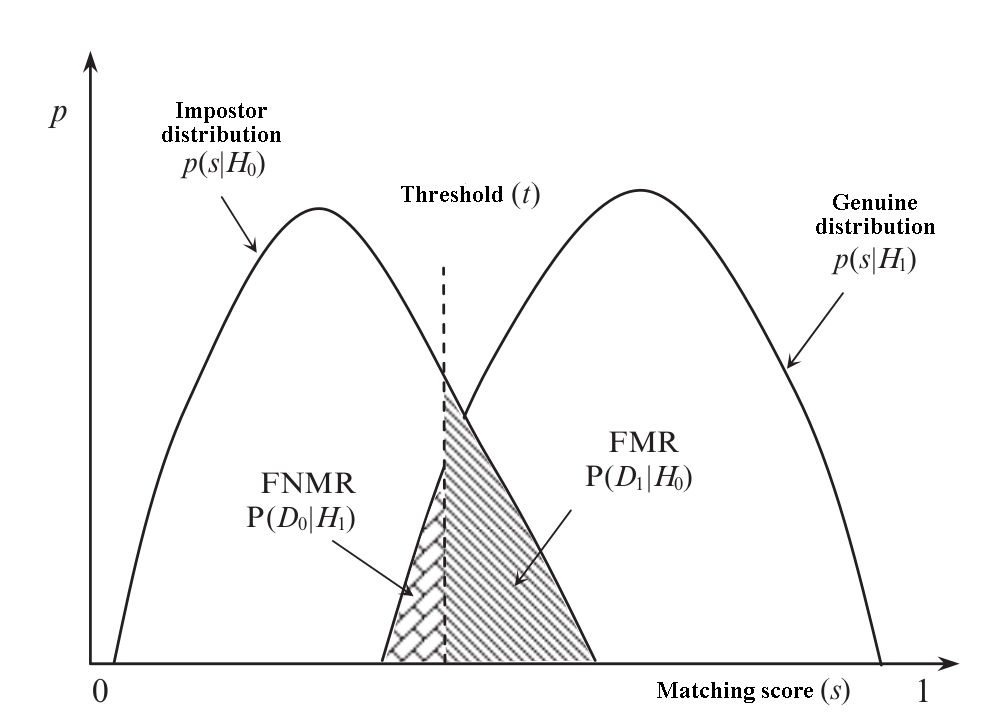
\includegraphics[width=0.7\linewidth]{obrazky-figures/fmr.png}}\\
        \caption{Graph FMR and FNMR. \cite{maltoni2009handbook}}
        \label{fig:fmr}
\end{figure}

\subsection{Attacks on biometric fingerprint systems}
Every biometric system has to consist of at least four modules which are sensor, feature extractor, matcher, and decision module. \cite{1262027} The schema of basic system can be seen in image \ref{fig:attack}. 

\begin{itemize}
	\item Sensors are described in section \ref{sensors}. 
	\item Feature extractor generates template based on extracted important data from raw data on input.
	\item Matcher is a module producing matching score, which stands for similarity of input biometric and biometric from the database generated by matching algorithm.
	\item The decision module compares the matching score with the threshold and decides on either accepting or rejecting biometric on an input.  
\end{itemize}\cite{1262027}

\begin{figure}[H]
    \centering
        {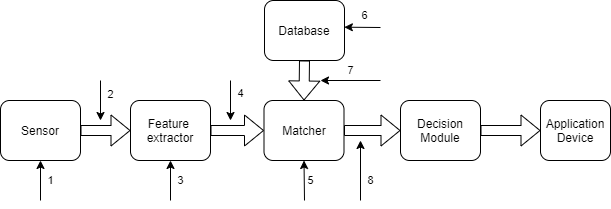
\includegraphics[width=\linewidth]{obrazky-figures/attack.png}}\\
        \caption{Attacks on the biometric system (numbered arrows shows points for possible attacks)}
        \label{fig:attack}
\end{figure}

There exist attack points not only in every module of a biometric system but also in every connection. There are 8 attack points show in figure \ref{fig:attack}. The attacks are divided into two basic groups: direct and indirect attacks.\cite{jain2015attacks}

Direct attacks do not require any knowledge about any other part of the system than the sensor. Attack on the sensor can be done with fake biometric (for example fake fingerprint made from gel, wax, ..) or just damaging the sensor itself.\cite{jain2015attacks}

Indirect attacks are the attacks where the impostor needs to know some information about the inner parts of the recognition system, which includes any of the parts (arrows with numbers) from figure \ref{fig:attack} except number 1, which is an attack on sensor.\cite{jain2015attacks}

While the sensor is sending raw data through a communication channel to a feature extractor for pre-processing it is possible to steal the biometric (point 2). The stolen biometric is later replayed to a feature extractor to bypass the sensor. To attack the feature extractor (point 3) the impostor pushes on output feature values except for the original ones. Attack on the communication channel between feature extractor and matcher (point 4) is similar to the attack on point 2 with the exception of stolen values.\cite{attack2}\cite{jain2015attacks}

Attack on matcher module is simply pushing on the output the desired value which can be the high score to pass the threshold or lower the score for the opposite result as same as just saying match or no match in cases where the decision is done already in a matching module.\cite{attack2} \cite{jain2015attacks}

Attack on the database (point 6) is as simple as pushing new or removing or modifying the existing templates in the existing database used by the biometric system. This attack is not easy as it seems, because saved templates are usually protected by steganography, watermarking, and other methods, which requires huge knowledge about the system. Another attack that can be done only while transmitting data from the database to the matcher is on point 7. This attack involves stealing, replacing, or altering biometric templates. \cite{mwema2015simple}\cite{jain2015attacks}

The last point where the impostor can be successful is on the communication channel between the matcher and the decision module (point 8). Although all the steps before were successful and well secured, the result can be still overridden, which causes the same result as attacking any point before.\cite{jain2015attacks}


\subsection{Morphing}
Morphing itself is the process of transformation between states of appearance. Basic operations used in morphing are translations rotations but it gets to harder operations like shapeshifting. \cite{morphing3} Image morphing has been shown as an extremely powerful tool not only for entertainment purposes. Morphing is mostly known as a technique that uses coupling image warping with color interpolation. Image warping is used for geometric transformation in 2D for maintaining feature alignment between features like the position of the nose and eyes. And the color interpolation is used for blending colors from input images.\cite{morphing2}\cite{morphing1}

The first step of morphing is finding the location of features from the input images. Then the primitives like mesh nodes, curves, or points are made correspondence between them is established. The primitives are established like that each is specifying one image feature or landmark. The second step is to compute the mapping function defying the special relationships between all points from both images. Mapping functions are used for interpolating positions while morphing two images together. After interpolation of positions, the color interpolation is run as the last step of morphing. \cite{morphing1}

In the past few years, big data and deep learning have become a trend, which can be seen even in morphing. For example, the generative adversarial network works for morphing well. The network is trained to synthesize frames by a given data-set of samples along the whole process of transformation. \cite{morphing3}

\section{Mathematical morphology}
In the last sixty years, there has been made huge progress in the area of image processing. The innovation is mostly in the meaning of transforming an image into a better-represented form in the next use, which can be image analysis or pattern recognition. The innovation never ends and very big attention is given to the field of mathematics morphology, because of its properties. The valued properties are quantitative descriptions of geometric structure and shape as well as a mathematical description of algebra, topology, probability, and integral geometry.\cite{shih2009image}

Mathematical morphology is having a huge impact on a lot of industries. Even in biology where it can be used on the extraction of forms or structures of animals or plants. Of course, it is used in the computer industry as well where it is mostly in computer vision for the extraction of representative components that can describe the whole topology or shape. There is a lot of mathematics used in morphology, the analysis is based on set theory, topology, lattice algebra, function, and many more.\cite{shih2009image}

Image is basically some multidimensional signal. The morphology was designed as complex as it can be. The morphological operations are that generally, that they can be used for analyzing any signal or even multidimensional geometric pattern.\cite{shih2009image}

\subsection{Binary morphology}
As written before the mathematical morphology is to help obtain or even obtain by itself some information. There are three described transformations: unary(one image on the input and one image on the output), dyadic (merging result to one image from two input images), and information extraction(one image on the input and information on the output). The binary stands for binary image what means that every pixel can contain only 2 values (in the basic 0 and 1). It is usually the rule that objects in front are with value 1 and objects in back has value 0. The advantage of binary images is that it has to store only pixels with value 1 because we know, that other pixels are 0 so we need to store only 2 values and that is the position (x, y). The advantage can be seen against the gray-scale image, where every element needs to store (x, y, z) where the z is the intensity of black color. On the other hand gray-scale stores more information, but in the extracted ridges, this information is useless.\cite{shih2009image}

\subsection{Binary dilation}
Minkowsky came first with the idea of dilation and it the reason why it can sometimes call Minkowsky complement. On this basis, we have our binary image on an input which is a set of positions. Then we combine our set with a template by use of the sum of the elements of the set. Definition is: Let $K$ and $L$ be two sets in $E^N$ with elements $k$ and $l$ in this order, where $k = (k_1, k_2, ..., k_N)$ and $l = (l_1, l_2, ..., l_N )$ stands for N-pairs positions of elements. Then the set of all possible vector sums of pairs of elements is the binary dilation $K$ by $L$, there one vector comes from $K$ and the other one from $L$. As described binary dilation works with binary images therefore is the name.\cite{shih2009image}


Let $K \subset E^N$ and $L \in E^N$. The shift $K$ by $L$, marked as $(K)_l$ is defined as: \cite{shih2009image} \cite{haralick1987image}
\begin{align}
    (K)_{l}=\left\{m \in E^{N} \mid m=k+l \quad \text { for some } k \in K\right\}
\end{align}

Let $K, L \subset E^N$. Binary dilation K o B, marked as $K \oplus_b L$, is defined as: \cite{shih2009image} \cite{haralick1987image}
\begin{align}
    K \oplus_{l} L=\left\{m \in E^{N} \mid m=k+l \quad \text { for any } k \in K \quad \text { k } l \in L\right\}
\end{align}

The set $K$ and set $L$ a having the symmetrical role. For a better understanding of the dilation here is the definition of local dilation (one step): Dilation $K \oplus_l L$ is the place of all centers $m$, in the way that shifts $(L)_m$, which is placed at the beginning $L$ in $m$, hits the set $K$.\cite{shih2009image}

\textbf{Properties of the dilation:}
\begin{align}
    &\text{If K contains beginning:} 0 \in L, \text{then} K \oplus L \supseteq K\\
    &\mathrm{K} \oplus_{l} L=L \oplus_{l} K\\
    &\left(K \oplus_{l} L\right) \oplus_{l} M=K \oplus_{l}\left(L \oplus_{l} M\right)\\
    &(K)_{x} \oplus_{l} L=\left(K \oplus_{l} L\right)_{x}\\
    &(K)_{x} \oplus_{l}(L)_{-x}=K \oplus_{l} L\\
    &\text { If } K \subseteq L, \text { then } K \oplus_{l} M \subseteq L \oplus_{l} M\\
    &(K \cap L) \oplus_{l} M \subseteq\left(K \oplus_{l} M\right) \cap\left(L \oplus_{l} M\right)\\
    &(K \cup L) \oplus_{l} M=\left(K \oplus_{l} M\right) \cup\left(L \oplus_{l} M\right)
    \cite{shih2009image}
\end{align}

\subsection{Binary erosion}
Erosion is based on the same principle, one input binary image, and one binary mask or core. Erosion is an opposite operation to the dilation where the vector subtraction of elements from the set. In simple way, lets $K$ and $L$ be sets in $E^N$ with elements $k$ and $l$. The erosion $K$ by $L$ is set of all the elements $x$ for which applies $x + k \in K$ and for all $l \in L$.\cite{shih2009image}

The definition of binary erosion $K$ by $L$ which is marked $A \ominus_b B$ is:\cite{dil1} \cite{dil2}
\begin{align} 
	K \ominus_l L = \{ x \in E^N | x+l \in K \textrm{ for each } l \in L \}
\end{align}

Another interpretation of binary erosion $K \ominus_l L$ can be a place of all centers $s$, so the shift $(L)_m$ is completely included in the set $K$. Definition in this case is:\cite{dil2}
\begin{align} 
K \ominus_l L = \{ m \in E^N | L_m \subseteq K \}
\end{align}

\textbf{Properties of the erosion:}

\begin{align}
    &\text{If L contains beginning: }0 \in L, then K \ominus_l L \subseteq K\\
    &\left(K \ominus_{l} L\right) \ominus_{l} M=K \ominus_{l}\left(L \oplus_{l} M\right)\\
    &K \oplus_{l}\left(L \ominus_{l} M\right) \subseteq\left(K \oplus_{l} L\right) \ominus_{l} M\\
    &K_{x} \ominus_{l} L=\left(K \ominus_{l} L\right)_{x}\\
    &\text { If } K \subseteq L, \text { then } K \ominus_{l} M \subseteq L \ominus_{l} M\\
    &(K \cap L) \ominus_{l} M=\left(K \ominus_{l} M\right) \cap\left(L \ominus_{l} M\right)\\
    &(K \cup L) \ominus_{l} M \supseteq\left(K \ominus_{l} M\right) \cup\left(L \ominus_{l} M\right)\\
    &K \ominus_{l}(L \cup M)=\left(K \ominus_{l} L\right) \cap\left(K \ominus_{l} M\right)\\
    &K \ominus_{l}(L \cap M) \supseteq\left(K \ominus_{l} L\right) \cup\left(K \ominus_{l} M\right)
    \cite{shih2009image}
\end{align}

The algebraic basis for mathematic morphology was introduced by Heijmans a Ronse \cite{heijmans1990algebraic}. As you could guess dilatation is not always reversible by erosion and conversely. $M = K \ominus_l L$ can be as example, when if erosion is used of both sides by L is having as result $M \ominus_l L = (K \oplus_l L) \ominus_l L \neq K$. So in the end the relation of closure $(K \oplus L) \ominus L \supseteq K$ is valid relation in this case. One interesting thing is that when the dilation and erosion are used clearly in binary image $K$ in structured element $L$, the index $l$ is omitted as can be seen in this relation. One example of binary erosion and dilation is shown in the picture\ref{fig:dil_morph}.

\begin{figure}[H]
    \centering
        {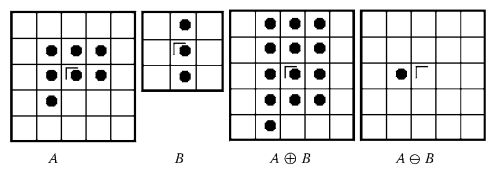
\includegraphics[width=0.8\linewidth]{obrazky-figures/dil_ero.png}}\\
        \caption{Binary dilation and erosion \cite{shih2009image}}
        \label{fig:dil_morph}
\end{figure}

\subsection{Thinning} \label{thinnin}
Thinning is a special kind of erosion. The main difference is in factors, which are: 1) the component in an image on the input can not disappear. 2) Output of thinning are 1 pixel wide objects, which means that the 1px wide line that is in the same distance from all the original edges (in the center). The structural shape of the object represented as a graph is an output of thinning. That is why it is used as a basic step in image processing in many industries like control of industrial parts or in our fingerprint detection. \cite{shih2009image}

The main use of thinning result which is the skeleton of an object is the representation and classification of the objects in the binary image. The first form of thinning was the definition of digital skeletons and algorithms based on set transformation and it was introduced by Jang and Chin \cite{jang1990analysis}. Another view on the thinning operation was introduced by Serra a Meyer \cite{serra1983image} \cite{serra1988mathematical} and their approach was based on operation "hit-or-miss" and in this approach the definition is: 
\begin{align}
K \wedge L=K-\left(K \mathrm{~s}^{*} L\right)=K \cap\left(K \mathrm{~s}^{*} L\right)^{m}
\end{align}\cite{serra1988mathematical}

The definition shows that thinning is basically nothing else than finding and deleting. All the presence of $L$ in $K$ are localized and subtracted by the operation $K s^* L$. All the elements that were found in $K$ are deleted. To complete the whole process of thinning, the sequence of structural elements is used: $\{K\}=\left\{L^{1}, L^{2}, \ldots, L^{8}\right\}$, where $K^{i}$ is turned version of $K^{i-1}$. In use on digital images and this implementation sequence of 8 elements is used:\cite{serra1988mathematical}

$$\begin{array}{l}
 
L^{1}=\left[\begin{array}{lll}
0 & 0 & 0 \\
\times & 1 & \times \\
1 & 1 & 1
\end{array}\right], 

\quad L^{2}=\left[\begin{array}{lll}
\times & 0 & 0 \\
1 & 1 & 0 \\
1 & 1 & \times
\end{array}\right], 

\quad L^{3}=\left[\begin{array}{lll}
1 & \times & 0 \\
1 & 1 & 0 \\
1 & \times & 0
\end{array}\right], 

\quad L^{4}=\left[\begin{array}{lll}
1 & 1 & \times \\
1 & 1 & 0 \\
\times & 0 & 0
\end{array}\right], \\

\\
L^{5}=\left[\begin{array}{lll}
1 & 1 & 1 \\
\times & 1 & \times \\
0 & 0 & 0
\end{array}\right], 

\quad L^{6}=\left[\begin{array}{lll}
\times & 1 & 1 \\
0 & 1 & 1 \\
0 & 0 & \times
\end{array}\right], 

\quad L^{7}=\left[\begin{array}{lll}
0 & \times & 1 \\
0 & 1 & 1 \\
0 & \times & 1
\end{array}\right], 

\quad L^{8}=\left[\begin{array}{lll}
0 & 0 & \times \\
0 & 1 & 1 \\
\times & 1 & 1
\end{array}\right]

\end{array}$$

Then the thinning by eight elements is defined as:\cite{shih2009image} \cite{serra1983image} \cite{serra1988mathematical}
\begin{align}K \wedge\{L\}=\left(\cdots\left(\left(K \wedge L^{1}\right) \wedge L^{2}\right) \cdots\right) \wedge L^{8}
\end{align}

In the process of thinning must be achieved erase of the edges under the condition that connectivity can not be changed. All eight cores are designed the way that they are together to meet the conditions. The process of using all eight cores is repeated until there is no change from the last step. The result of thinning is shown in image \ref{fig:dil_thin} \cite{shih2009image}

\begin{figure}[H]
    \centering
        {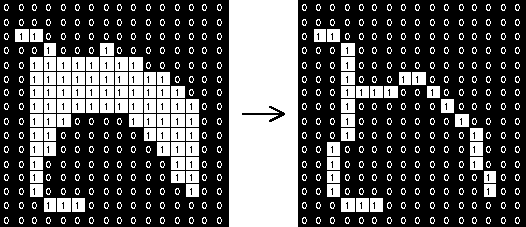
\includegraphics[width=0.8\linewidth]{obrazky-figures/thinning.png}}\\
        \caption{Thinning \cite{Morpholo62:online}}
        \label{fig:dil_thin}
\end{figure}

\section{Digital image processing}
Image processing is used to extract some useful information or get an enhanced image from the image on an input. The use of image processing has been increasing exponentially in the last decades and it is being used from entertainment to medicine. \cite{imageProcessing}

Digital image processing is a huge field and it consists of encompassing digital signal processing techniques and specific techniques to image. Image can be described as function f(x,y), where x and y are continuous variables. It has to be sampled and transformed into a matrix of numbers for digital processing. So the digital image processing stands for manipulation with these finite numbers. There are several types of image processing:\cite{imageProcessing}

\begin{itemize}
	\item \textbf{image enhancement:} Image is manipulated mostly by heuristic techniques and it is easier to extract the information from the result.
	\item \textbf{image restoration:} Processing of damaged images which is trying to find statistical or mathematical descriptions of degradation to revert the degradation.
	\item \textbf{image analysis:} processing of an image for automatic extraction of information. (examples are image segmentation or edge extraction)
	\item \textbf{image compression:} compression applied on digital images with a goal to reduce their cost for transmission and storage.
\end{itemize}\cite{imageProcessing}

\subsection{Histogram equalization}
Histogram equalization is a technique for adjusting image intensities to enhance contrast. The histogram is a graphical representation of the intensity distribution of an image. Enhancing image contrast is accomplished by spreading out the most frequent intensity values. The global contrast is usually increased by this technique where the data on an input were represented with very close contrast. \cite{histogram}

\begin{figure}[H]
    \centering
        {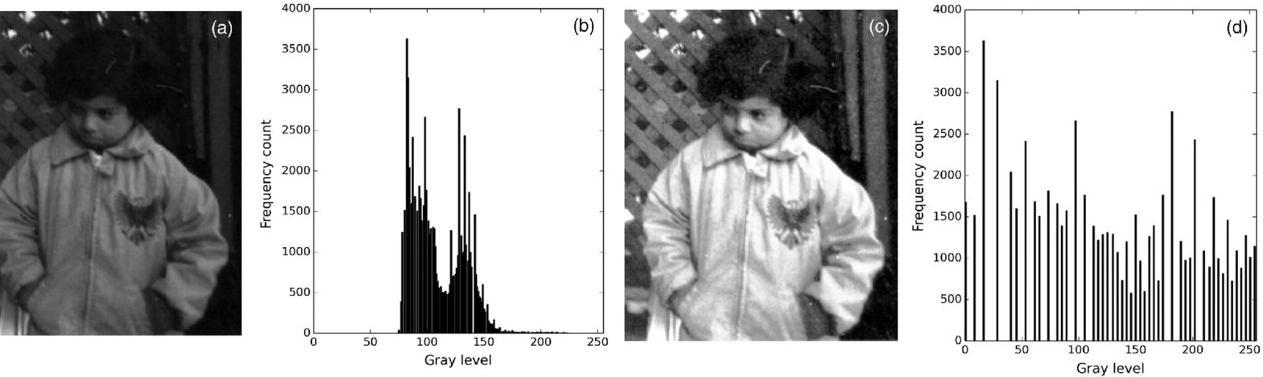
\includegraphics[width=0.8\linewidth]{obrazky-figures/histogram.png}}\\
        \caption{Histogram equalization: a)input image, b) input image histogram, c)input image after histogram equalization d)input image histogram after equalization\cite{histogram}}
        \label{fig:histogram_eq}
\end{figure}

\subsubsection{Contrastive Limited Adaptive Equalization (CLAHE)}
The technique of histogram equalization is having problems with over-amplification of noise. Therefore the separate histograms are calculated in adaptive histogram equalization (AHE). AHE can achieve higher contrast enhancement, but because some homogeneous regions may be oversaturated, it amplifies the noise. Therefore the amplification is limited by clipping the histogram at a predefined value in the CLAHE algorithm. \cite{histogram}


\label{suggestion}
\chapter{The suggestion of solution}
This chapter describes the techniques needed to create morphed fingerprints. For certain parts, such as thinning, it is necessary to know the theory described in the chapter \ref{theory}.

\section{Fingerprint image preprocessing}\label{preprocessing}
The first step is to convert the fingerprint image from input to the gray-scale image. The papillary lines are thus marked in darker gray in the figure and the valley in white or lighter shades of gray. First, so that we do not work on unnecessarily large fingerprint images, the detection of fingerprint boundary points (leftmost point, lowest point, ..) and subsequent trimming of the excess background is performed. For subsequent processing, a fingerprint mask is calculated in the same step. For the most realistic results of morphing, it is necessary to ensure the highest possible similarity between prints before its implementation, and therefore the color normalization is performed using the minimax algorithm, where there is a linear mapping to the interval between min and max.

\section{Fingerprints alignment}
To find the best position to align two fingerprints on top of each other, a technique based on oriented fields is used. The use of kernel or delta alignment has also been considered, but some fingerprints are very different and a similar implementation would then not work properly.

\subsection{Algorithm for fingerprint orientation field} \label{oricomp}
Let $[x, y]$ be a pixel in the fingerprint image. Then the angle $\theta_{x,y}$ is a local orientation of all the ridges in pixel $[x, y]$ that are coming through the arbitrarily large surroundings centered in pixel $[x, y]$. $\theta_{x,y}$ is in the range $[0..\pi]$ just because the ridges have no direction. Then the fingerprint orientation field is matrix D, in which the elements store the local orientation of the ridges in the given surroundings. Each element $ \theta_{x, y} $ of the matrix D indicates the average orientation of the lines around the pixel $[x, y]$, where the pixel $[x, y]$ represents the square grid located above this point. The result fingerprint orientation field can be seen in the image \ref{fig:ori_img}. Each element $ \theta_{x, y} $ is often associated with a value of $ r_{x, y} $, which indicates the degree of reliability of the orientation.\cite{ori}

\begin{figure}[H]
    \centering
        {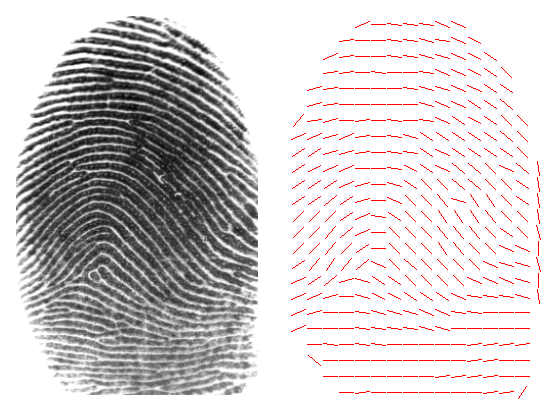
\includegraphics[width=0.5\linewidth]{obrazky-figures/ori_navrh.png}}\\
        \caption{Input fingerprint image on the left side, fingerprint orientation field on the right side}
        \label{fig:ori_img}
\end{figure}

Algorithm description:

\begin{enumerate}
	\item In the beginning, the normalized image $\mathcal{G}$ needs to be divided into w*w blocks. Then there is no ridge in the block, value 0 is assigned and r is set to 0 as well otherwise the r is set to 1 and the calculation can begin. \cite{ori}
	
	\item For each pixel (x,y) the gradients  $\partial_{i}(x, y)$ and $\partial_{j}(x, y)$ needs to be computed by the Sobel operator.\cite{ori}
	
	  \item The local orientation is set for each block with center in pixel (x, y), by these equations:\cite{ori}
        \begin{equation} 
            \mathcal{V}_{i}(x, y)=\sum_{u=x-\frac{w}{2}}^{x+\frac{w}{2}} \sum_{v=y-\frac{w}{2}}^{y+\frac{w}{2}} 2 \partial_{i}(u, v) \partial_{j}(u, v)
        \end{equation}
        \begin{equation} 
            \begin{split}
                \mathcal{V}_{j}(x, y)=\\\sum_{u=x-\frac{w}{2}}^{x+\frac{w}{2}} \sum_{v=y-\frac{w}{2}}^{y+\frac{w}{2}}\left(\partial_{i}^{2}(u, v)-\partial_{j}^{2}(u, v)\right)
            \end{split}
        \end{equation}
        \begin{equation} 
            \theta(x, y)=\frac{1}{2} \tan ^{-1}\left(\frac{\mathcal{V}_{j}(x, y)}{\mathcal{V}_{j}(x, y)}\right)
        \end{equation}
        
        Where $\theta(x, y)$ is the smallest square estimation of the local orientation of the ridges in the block centered at (x, y).
         
	\item To remove or at least reduce errors that cause noise or other, the low pass filter can be used. It can be used because of the low variability of ridges in the near surroundings except around the singular points. Before filtration every $\theta(x, y)$ needs to be converted into the vector field. Equation of conversion to vector field:\cite{ori}
    \begin{equation}
         \Phi_{i}(x, y)=\cos (2 \theta(x, y))
    \end{equation}   
    \begin{equation}
         \Phi_{j}(x, y)=\sin (2 \theta(x, y))
     \end{equation}\cite{ori}
     The filtration with low pass filter:\cite{ori}
     \begin{equation}
         \begin{split}
             \Phi_{i}^{\prime}(x, y)= \sum_{u=-w_{\Phi} / 2}^{w_{\Phi} / 2} \sum_{v=-w_{\Phi} / 2}^{w_{\Phi} / 2} \\ W(u, v) \Phi_{i}(x-u w, y-v w)
        \end{split}
     \end{equation}
     \begin{equation}
        \begin{split}
             \Phi_{y}^{\prime}(x, y)=\sum_{u=-w_{\Phi} / 2}^{w_{\Phi} / 2} \sum_{v=-w_{\Phi} / 2}^{w_{\Phi} / 2} \\ W(u, v) \Phi_{j}(x-u w, y-v w)
        \end{split}
     \end{equation}
	Where the $W$ is a low pass filter. In default, 5x5 is the size of the filter.   
	
     \item 
     The computation of the smoothed local orientation is then performed using equation:
      \begin{equation}
        \mathcal{O}(x, y)=\frac{1}{2} \tan \left(\frac{\Phi_{j}^{\prime}(x, y)}{\Phi_{i}^{\prime}(x, y)}\right)
     \end{equation}
\end{enumerate}\cite{ori}

After computing the oriented field for both fingerprints, it is finally possible to start aligning them. The method tries to maximize the similarity of oriented fields at their intersections.

The oriented fields $ \mathcal{O}_1 $ and $ \mathcal{O}_2 $ are calculated in blocks w x w and at each position (x, y) it contains the value of the size of the angle $ \theta $ and r = [0,1]. Then the similarity between oriented arrays is calculated: \cite{morphing_paper} 	

\begin{equation}
\begin{split}
S\left(\mathcal{O}^{1}, \mathcal{O}^{2}\right)=\\
\frac{\sum_{(x, y) \in\left(V_{\mathcal{O} 1} \cap V_{\mathcal{O} 2}\right)}\left(r_{x, y}^{y}+r_{x, y}^{2}\right) \cdot \psi\left(\theta_{x, y}^{1}, \theta_{x, y}^{2}\right)}{\sum_{(x, y) \in\left(V_{\mathcal{O}^{1}} \cap V_{\mathcal{O}^{2}}\right)}\left(r_{x, y}^{1}+r_{x, y}^{2}\right)}
\end{split}
\end{equation}

, where $\psi\left(\theta_{1}, \theta_{2}\right) $ is the similarity of orientation fields:
\begin{equation}
\psi\left(\theta_{1}, \theta_{2}\right)=1-\frac{2 \cdot\left|\theta_{1}-\theta_{2}\right|}{\pi}
\end{equation}

and positions of the front are included in $V_{\mathcal{O}}$:
\begin{equation}
V_{\mathcal{O}}=\left\{(x, y) | o_{x, y} \in \mathcal{O} \wedge r_{x, y}>0\right\}
\end{equation}\cite{morphing_paper}

The alignment is computed for every position and angle the positions are skipped for positions of oriented fields on which they do not overlap sufficiently (at least $25\%$ overlap).\cite{morphing_paper}

\begin{equation}
\frac{\left|V_{\mathcal{O}^{1}} \cap V_{\mathcal{O}}\right|}{\max \left(\left|V_{\mathcal{O}^{1} }\right|, | V_{\mathcal{O}^{2} }|\right)} \geq min_{V R}
\end{equation}\cite{morphing_paper}

In my implementation, I only consider rotation in the range $ <-\pi/2; \pi/2> $ and a shift of a maximum of 50 \% of the width when moving right or left and 50 \% of the height when moving up or down. Larger changes either led to inaccuracies or did not affect the result. Furthermore, I always try to put a smaller fingerprint on a larger one. After aligning the prints, parts that are not intersecting are trimmed. An example of the result is in image \ref{fig:prunik}.
\begin{figure}[H]
    \centering
        {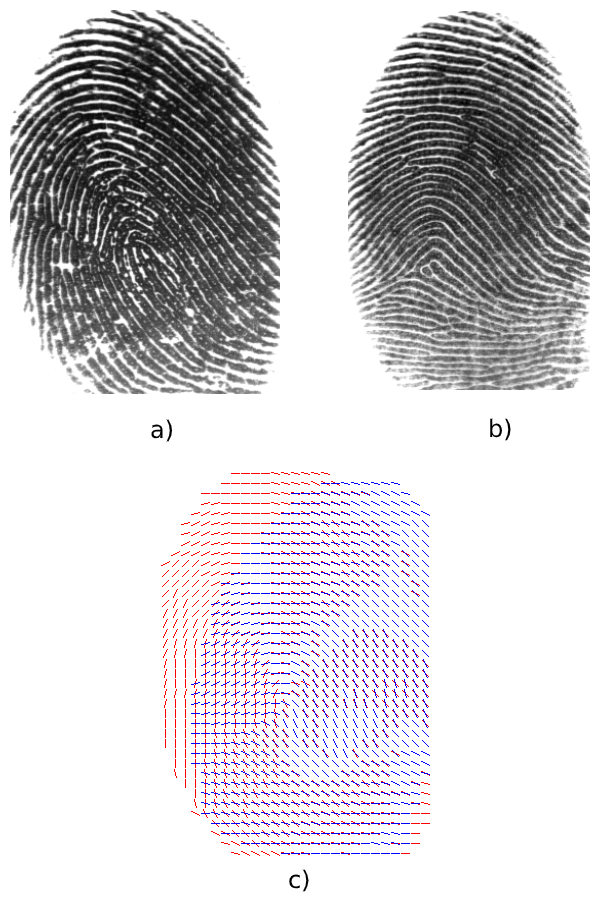
\includegraphics[width=0.5\linewidth]{obrazky-figures/prunik.png}}\\
        \caption{a)fingerprint 1 b) fingerprint 2 c) aligned fingerprint orientation fields}
        \label{fig:prunik}
\end{figure}

\section{Ridge frequency image}
It is possible to model levels of gray as sine waves in the near neighborhood of the fingerprint. This can be applied only in cases where no singular point is present in the examined neighborhood. For these cases, the frequency from near neighborhoods will be used. The definition and equations:
Let's have $ \mathcal{G} $ denoting the normalized fingerprint image and $\mathcal{O}$ oriented field calculated as described in the previous section. Then: \cite{ori}


\begin{enumerate}
    \item The fingerprint image ($\mathcal{G}$) is divided into blocks with size $w \times w$ usually 16 $\times$ 16. The block size has to be the same as block size for the fingerprint orientation field($\mathcal{O}$).\cite{hong1998fingerprint}
    
    \item Compute an \emph{oriented window}(something else then \ref{oricomp}) with size $l \times w$ usual size is 32 $\times$ 16 for each block centered at $(x, y)$.\cite{hong1998fingerprint}
    
    \item Compute the x-signature $X[0], X[1], ... X[l-1]$ of ridges inside oriented window for every block centered in $(x, y)$, where:
    \begin{align}
    X[k]=\frac{l}{w} \sum_{d=0}^{w-1} \mathcal{G}(u, v), \quad k=0,1, \ldots, l-1 \\
    u=x+\left(d-\frac{w}{2}\right) \cos \mathcal{O}(x, y)+\left(k-\frac{l}{2}\right) \sin \mathcal{O}(x, y)\\
    v=y+\left(d-\frac{w}{2}\right) \sin \mathcal{O}(x, y)+\left(\frac{l}{2}-k\right) \cos \mathcal{O}(x, y)
    \end{align}
	In the case where no singularity or minutiae is not present in the oriented window, x-signature creates a sin curve and frequency can be counted from it. Let the average count of pixels between two ridges be $\mathcal{T}(x, y)$. Then the equation for frequency $\Omega(x, y)$ is: $\Omega(i, j)=1 / \mathcal{T}(i, j)$. Value -2 is assigned if no ridge is found in the oriented window, so it is marked as non-valid.\cite{hong1998fingerprint}
    
    \item The ridge frequency in fingerprint images lies in a certain range. In the most common resolution, o 500dpi the range is $[ 1/3, 1/25]$. This range is used to check if the value is valid, if the frequency is not laying in this range then -1 is assigned as non-valid frequency.\cite{hong1998fingerprint}
    
    \item For blocks in which a singularity or landmark appears, the value must be calculated by interpolating the frequencies of adjacent blocks. The interpolation is performed as follows:\cite{hong1998fingerprint}
    
    \textbf{Step 1:}For each block with center at $(x, y)$,
    \begin{align}
        \Omega^{\prime}(x, y)=\left\{\begin{array}{ll}
        \Omega(x, y), & \text { if } \Omega(x, y) \neq-1 \\
        \frac{\sum_{u=-w_{\Omega} / 2}^{w_{\Omega} / 2} \sum_{v=-w_{\Omega} / 2}^{w_{\Omega} / 2} W_{g}(u, v) \mu(\Omega(x-u w, y-v w))}{\sum_{u=-w_{\Omega} / 2}^{w_{\Omega} / 2} \sum_{v=-w_{\Omega} / 2}^{w_{\Omega} / 2} W_{g}(u, v) \delta(\Omega(x-u w, y-v w)+1)} & \text { otherwise }
        \end{array}\right.
    \end{align}
        where
    \begin{align}
        \begin{aligned}
        \mu(a) &=\left\{\begin{array}{ll}
        0, & \text { if } a \leq 0 \\
        a, & \text { otherwise }
        \end{array}\right.\\
        \delta(a) &=\left\{\begin{array}{ll}
        0, & \text { if } a \leq 0 \\
        1, & \text { otherwise }
        \end{array}\right.
        \end{aligned}
    \end{align}
	
	$W_g$ stands for discrete Gaussian filter, where size of the filter is: $w_\Omega = 7$, mean has value of 0 and variance is 9.\cite{hong1998fingerprint}
    
    \textbf{Step 2:} Repeat step 1 until the is one frequency in the image with value -1, before repetition swap $\Omega$ and $\Omega'$
    
    \item Similarly, as with the fingerprint orientation field, the low pass filter can be used to remove outliers. This can proceed because the frequency is changing really slowly in the near neighborhood:
    \begin{align}
        F(x, y)=\sum_{u=-w_{\Omega} / 2}^{w_{l} / 2} \sum_{v=-w_{\Omega} / 2}^{w_{l} / 2} W_{l}(u, v) \Omega^{\prime}(x-u w, y-v w)
    \end{align}
	
	$W_l$ stands for the low pass two dimensional filter with unit integral and size $w_l = 7$. \cite{hong1998fingerprint}
	
\end{enumerate}
\begin{figure}[H]
    \centering
        {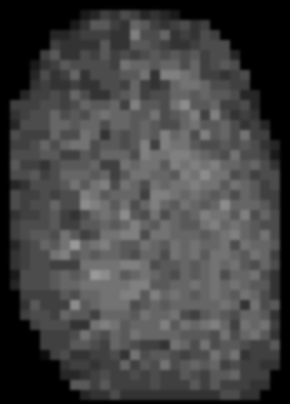
\includegraphics[width=0.3\linewidth]{obrazky-figures/freq_navrh.png}}\\
        \caption{Ridge frequency image of fingerprint from image \ref{fig:ori}}
        \label{fig:freq_img}
\end{figure}

\section{Minutiae}
The application uses an algorithm working on the extraction of minutiae with the use of thinning. To extract the minutiae, it is necessary to first calculate the oriented field described above. Then distinguish the background and the fingerprint. An important step is the extraction of ridges and creates a binary image, where the ridges carry the value 1. The last step of line extraction is thinning, see \ref{thinnin}.

Subsequent extraction of the minutiae is performed by using the crossing number method on the neighborhood of the point P at a distance of 1. Or on its 8 surrounding pixels:\cite{thinning}

\begin{equation}
    C N=0.5 \sum_{i=1}^{8}\left|P_{i}-P_{i+1}\right|, \quad P_{9}=P_{1}
\end{equation} .

Subsequently, false markers will be removed in post-processing. The first part is ridge counting. Ridge counting determines how many lines pass through or touch the line that connects the core and delta. For this operation, it is necessary to determine the delta and the core of the fingerprint as accurately as possible. Then:

\begin{itemize}
	\item If ridge bifurcation lays on the ridge, then two ridges are counted
	\item If the ridge is touching the island or dot, then one ridge is counted.
    \item The valley must be interrupted by a line between the delta and the core, otherwise, one line is subtracted. (Applies to loop lines only.)\cite{thinning}
\end{itemize}

In the end, the minutiae validity needs to be checked. The check is made by distance measurement: Firstly the average count of pixels between 2 ridges is counted (ridge counting distance = RCG). Secondly, the distance between delta and core (DC) is counted. Then the distance of minutiae from the next minutiae has to be larger than RCG/DC.\cite{thinning}

\section{The cutline estimation}
This is the line around which most minutiae occur and when generating a new fingerprint, it ensures that there will be a sufficient number of minutiae from both fingerprints in the newly generated fingerprint. The straight line is calculated after performing all previously described operations, so it is computed from aligned and truncated impressions from parts of the non-intersection and with their oriented fields. Minutiae extracted from these prints are denoted as $T^1$ for fingerprint 1 and $ T^2 $ for fingerprint 2.\cite{morphing_paper}

The $ \rho = (\rho_x, \rho_y) $ is assigned as a barycenter. The article does not say what exactly it is, so I used the core or delta if cores is not present. \cite{morphing_paper}

Then the cutline $l$ has these paramtres:\cite{morphing_paper}
\begin{equation}
    \begin{array}{l}
    a_{l} \cdot x+b_{l} \cdot y+c_{l}=0 \\
    a_{l}=\sin (\beta), \quad b_{l}=\cos (\beta) \\
    c_{l}=-\rho_{x} \cdot \sin (\beta)-\rho_{y} \cdot \cos (\beta)
    \end{array}
\end{equation}

Now the line is rotated around the barycenter by a predetermined step in the range $ (0^{\circ}, 180^{\circ}) $. A straight line score $S_(c)$ is specified for each $\beta$ angle: \cite{morphing_paper}

\begin{equation}
    S_{c}=\omega_{o} \cdot S_{o}+\omega_{v} \cdot S_{v}+\omega_{m} \cdot S_{m}
\end{equation}

Where $S_o$ is the similarity of the oriented fields, $S_v$ is the similarity of the frequency characteristics, $S_m$ is the score used to evaluate the generation of a fingerprint similar to both based on the found minutiae of fingerprint 1: $ T_1 $, and fingerprint 2: $ T_2 $. $ \omega_{o}, \omega_{v}, \omega_{m} $ are then the weights of individual components in the range $ <0; 1> $, $ \omega_{o} + \omega_{v} + \omega_{m} = 1$. \cite{morphing_paper}

\begin{equation}
    S_{o}=\frac{\sum_{(i, j) \in C}\left(r_{i, j}^{1}+r_{i, j}^{2}\right) \cdot \psi\left(\theta_{i, j}^{1}, \theta_{i, j}^{2}\right)}{\sum_{(i, j) \in C}\left(r_{i, j}^{1}+r_{i, j}^{2}\right)}
\end{equation}
\begin{equation}
    S_{v}=\frac{\sum_{(i, j) \in C}\left(1-\frac{\left|v_{i, j}^{1}-v_{i, j}^{2}\right|}{\left(\max _{F}-\min _{F}\right)}\right)}{|C|}
\end{equation}

Only the elements that are in the intersection of oriented fields and their distance is maximal $d_{max}$ from actual cutline $l$ is in the $C$. So:

\begin{equation}
  \begin{split}
      C=\{(i, j) |(i, j) \in\left(V_{\hat{O}^{1}} \cap V_{\hat{O}^{2}}\right) \wedge \\\operatorname{dist}_{l}(i, j) \leq d_{\max }\}
  \end{split}
 \end{equation}
 \begin{equation}
     \operatorname{dist}_{l}(x, y)=\frac{\left|a_{l} \cdot x+b_{l} \cdot y+c_{l}\right|}{\sqrt{a_{l}^{2}+b_{l}^{2}}}
 \end{equation}
 \begin{equation}
     S_{m}=\max \left(\zeta_{m}\left(T^{1}, T^{2}\right), \zeta_{m}\left(T^{2}, T^{1}\right)\right)
 \end{equation}
 \begin{equation}
 \begin{split}
     \zeta_{m}(A, B)=\\\frac{Z\left(|A|_{l}^{P}, \mu_{m}, \tau_{m}\right)+Z\left(|B|_{l}^{N}, \mu_{m}, \tau_{m}\right)}{2}
 \end{split}
 \end{equation}
 where the $|T|_{l}^{P}$ stands for minutiae which are over the cutline (from the first fingerprint) and $|T|_{l}^{N}$ stand for minutiae under the cutline. So:
 \begin{equation}
     \begin{array}{l}
        |T|_{l}^{P}=\left|\left\{m \in T | \phi_{l}\left(m_{x}, m_{y}\right) \geq 0\right\}\right| \\
        |T|_{l}^{N}=\left|\left\{m \in T | \phi_{l}\left(m_{x}, m_{y}\right)<0\right\}\right|
    \end{array}
 \end{equation}\cite{morphing_paper}

The result needs to be normalized into the range $<0;1>$. Therefore the sigmoid function Z is and is controlled by the parameters $\mu$ a $\tau$. \cite{morphing_paper}
\begin{equation}
    Z(v, \mu, \tau)=\frac{1}{1+e^{-\tau(v-\mu)}}
\end{equation}
As the result cutline is assigned cutline with highest score $S_c$.\cite{morphing_paper}
 
\label{imageBased1}
\section{Image-based fingerprint generation} \label{picgen}
The fingerprint is generated by merging fingerprint intersections. Let $ \hat{F}^{p} $ be the part of the fingerprints above the cutline and $ \hat{F}^{n} $ be the part of the fingerprints below the cutline, which we determine as follows:
\begin{equation}
    (p, n)=\left\{\begin{array}{ll}
    (1,2) & \text { if } \zeta_{m}\left(T^{1}, T^{2}\right) \geq \zeta_{m}\left(T^{2}, T^{1}\right) \\
    (2,1) & \text { otherwise }
    \end{array}\right.
\end{equation}\cite{morphing_paper}

Then the fingerprint generation looks like: 
\begin{equation}
    D^{I}(x, y)=w_{x, y}^{l_{\max }} \cdot \hat{F}^{p}(x, y)+\left(1-w_{x, y}^{l_{m a x}}\right) \cdot \hat{F}^{n}(x, y)
\end{equation}\cite{morphing_paper}
where $w_{x, y}^{l_{\max }}$ is weight to balance the mixing in near distance to the cutline.\cite{morphing_paper}
    
\begin{equation}
    w_{x, y}^{l_{\max }}=\left\{\begin{array}{c}
    1-\max \left(0, \frac{d_{\max }-\operatorname{dist}_{\max }(x, y)}{2 \cdot d_{\max }}\right) \\
    \operatorname{if} a_{\ln a x} \cdot x+b_{\ln a x} \cdot y+c_{\ln a x} \geq 0 \\
    \max \left(0, \frac{d_{\max }-\operatorname{dist}_{\ln a_{a x}}(x, y)}{2 \cdot d_{\max }}\right) \text { otherwise }
    \end{array}\right.s
\end{equation}

\label{imageBased2}
\section{Improved image based generation}
After going through image-based generation from the previous section \ref{imageBased1} some ideas have been shown. Some improvements were made in steps after generation and mostly to make the generation more universal to different fingerprints. The first improvement was made on the computation of the mask for fingerprint. Since the given database contains fingerprints scanned with some noise, maximal movement in pixels had to be added to avoid containing it in mask, where the optimal value was considered as 5px.

The main change making the most of improvement is rotating the cutline around the center of the first fingerprint. The option of rotating the cutline around the core or delta can lead to maximalize only one fingerprint on the whole image based on the position of the core or delta on the fingerprint. This can be seen in the example from picture \ref{fig:bad_show}.

\begin{figure}[H]
    \centering
        {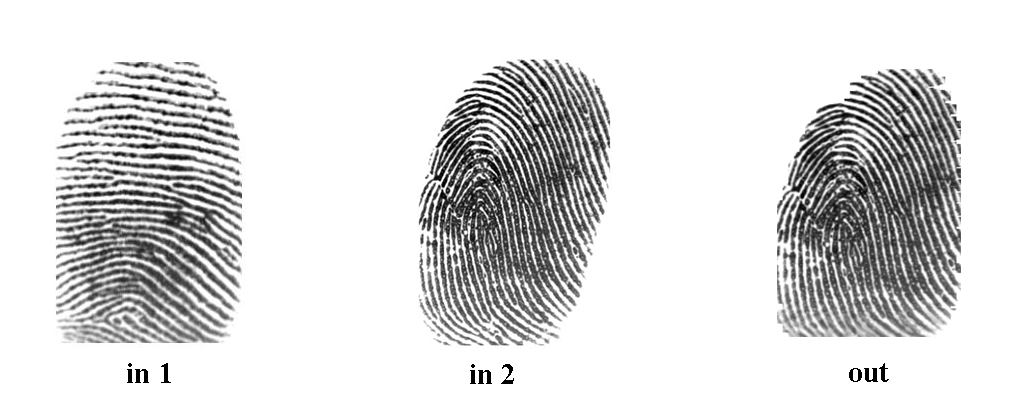
\includegraphics[width=1\linewidth]{obrazky-figures/bad_show.png}}\\
        \caption{Demonstration of fingerprint generation problem (in1, in2 = input fingerprints, out = morphed fingerprint). Only small part at bottom is contained from fingerprint in1}
        \label{fig:bad_show}
\end{figure}

Putting barycenter into the center deletes this kind of mistake. But also brings one for the human eye. The fingerprints can contain more than one core this way. And sometimes are easily discovered as fake by the human eye.

The next idea that proved to be right was to apply contrast limited adaptive histogram equalization (CLAHE) after the whole fingerprint generation. Since the given database is containing fingerprints that differ a bit more in contrast. The CLAHE makes these differences less visible.

The last change made was going over the result with the Gaussian filter with kernel 5x5 to blur a bit the whole fingerprint and make less visible the transitions between fingerprints. This option works properly only in some cases and is not included in final testing.

\section{Minutiae-based fingerprint generation}
To complete all ideas about fingerprint image generation the second fingerprint generation from paper \cite{morphing_paper} is mentioned as well. But because of different topics and the author’s tests against VeriFinger which ended worse than image-based morphing, this solution was neither implemented or tested. 

A realistic fingerprint can be generated synthetically based on features with a combination of fingerprint orientation fields and frequencies. The first step is to obtain dual identity fingerprint information ($ \tilde{O} $ orientation field, $ \tilde{\Upsilon} $ frequency field and $ \tilde{T} $ markers) by combining the first and second fingerprints similar to the method \ref{picgen}. \cite{morphing_paper}

\begin{equation}
    \tilde{O}(x, y)=w_{x, y}^{l_{\max }} \cdot \hat{O}^{p}(x, y)+\left(1-w_{x, y}^{l_{\max }}\right) \cdot \hat{O}^{n}(x, y)
\end{equation}
\begin{equation}
    \tilde{\Upsilon}(x, y)=w_{x, y}^{l_{\max }} \cdot \Upsilon^{p}(x, y)+\left(1-w_{x, y}^{l_{\max }}\right) \cdot \Upsilon^{n}(x, y)
\end{equation}
\begin{equation}
\tilde{T}=\left\{m \in T^{p}, \phi_{l_{\max }}\left(m_{x}, m_{y}\right) \geq 0\right\} 
\cup\left\{m \in T^{n}, \phi_{l_{\max }}\left(m_{x}, m_{y}\right)<0\right\}
\end{equation}

The generation itself is based on two steps:

\begin{enumerate}
    \item In the first step, we work only with minutiae and fingerprint orientation field from the input, which carry information about the position $ x_i, y_i $ and the type of marker. We recognize only two types of minutiae and that is the bifurcation and the ridge ending. Then the minutiae are placed in position according to the position and turn it by an angle according to the field of orientations.\cite{syntetic_gen_paper}
    
    \item In the second step, the papillary lines are "grown" from the markers using a Gabor filter modified to work with the frequency field $v$ and the fingerprint orientation field $ \ phi_{x y} $:\cite{syntetic_gen_paper}
    \begin{equation}
        \text{gabor}\left(r, s: \phi_{x y}, \nu\right)=e^{-\frac{(r+s)^{2}}{2 \sigma^{2}}} \cdot \cos \left[2 \pi \nu\left(r \sin \phi_{x y}+s \cos \phi_{x y}\right)\right]
    \end{equation}
\end{enumerate}

In the end, it is possible to crop the fingerprint to the shape of the fingerprint and add a little noise to make it "real" for the human eye as well. Trimming will be performed according to the mask calculated in the section\ref{preprocessing}.

\begin{figure}[H]
    \centering
        {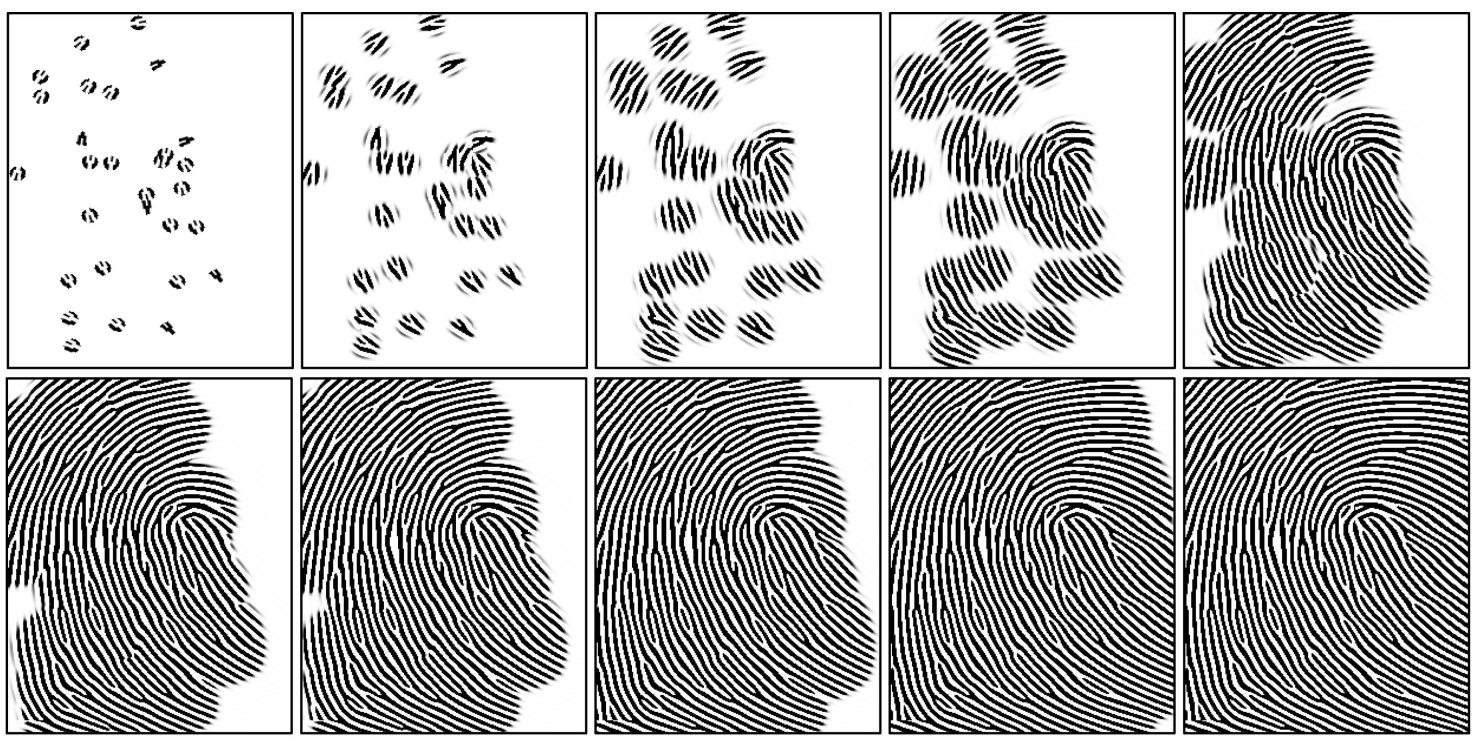
\includegraphics[width=1\linewidth]{obrazky-figures/gen2.png}}\\
        \caption{Demonstration of fingerprint generation \cite{syntetic_gen_paper}}
        \label{fig:syn}
\end{figure}

\chapter{Implementation}
This chapter describes the implementation of both morphing applications and fingerprint matching applications with the use of tools from Innovatrics and Neurotec. A laptop with the following configuration was used for testing:
\begin{itemize}
    \item CPU: Intel Core i5-6200U
    \item RAM: 8GB DDR4
    \item SSD: SSD 2400s M.2 2280 128GB
    \item OS: Windows 10
\end{itemize}

\label{mainmorph}
\section{Morphing application}
The application for morphing was implemented in Python version 3.8.5. as a console application with the use of these libraries: NumPy, SciPy, PIL, Matplotlib, OpenCV, and one GitHub repository, which was used for minutiae detection and thinning. The application is generating one morphed fingerprint from two fingerprints on the input based on an algorithm described in chapter \ref{suggestion}. 

The application runs on two modes first is for just to generate one morphed result, second is to generate all results from folders on an input. Both needs to get set \texttt{-{}-blocksize} or optionally \texttt{-{}-center}, \texttt{-{}-plot} or \texttt{-{}-save}. First then needs to get set input images (\texttt{-{}-image\_1} and \texttt{-{}-image\_2}). The second needs to get set input folders (\texttt{-{}-filder1}, \texttt{-{}-folder2} and \texttt{-{}-folder3}) and suffix of input images (\texttt{-{}-suf}).

\subsubsection{Application control}
\texttt{python morph.py [-h] [-{}-image\_1 /path/to/first/fingerprint/image/]} \\ \texttt{[-{}-image\_2 /path/to/second/fingerprint/image/] -{}-blocksize int [-{}-save \\ filename] [-{}-folder1 folder] [-{}-folder2 folder] [-{}-folder3 folder] [-{}-plot]} \\ \texttt{[-{}-suf .bmp/ .tif /...] [-{}-center]}

\begin{itemize}
    \item \texttt{-h}: Show help 
    \item \texttt{-{}-image\_1 /path/to/first/fingerprint/image/}: First input image for morphing. Only for one generation.
    \item \texttt{-{}-image\_2 /path/to/second/fingerprint/image/}: Second input image for morphing. Only for one generation.
    \item \texttt{-{}-blocksize int}: Integer value for blocksize
    \item \texttt{-{}-save filename}: Save to file filename. If not set, nothing is saved.
    \item \texttt{-{}-folder1 folder}: Folder with first input images. Argument used only for generating over whole folder.
    \item \texttt{-{}-folder2 folder}: Folder with second input images. Argument used only for generating over whole folder.
    \item \texttt{-{}-folder2 folder}: Folder for output images. Argument used only for generating over whole folder.
    \item \texttt{-{}-plot}: Plots few steps with Matplotlib. Steps: 
    Input images without background, orientation fields, alligned fingerprints, frequency image and minutiae, optimal cutline with barycenter and result. Demonstration of output can be seen in figure \ref{fig:app_plot}
	\item \texttt{-{}-suf .bmp/.tif /...}: Suffix of files in the folders that should be taken as an input.
	\item \texttt{-{}-center}: Take center of fingerprints as a barycenter for cutline
	\item \texttt{-{}-eq}: Use CLAHE on result
	\item \texttt{-{}-gaus}: Use gaussian blur on result
\end{itemize}

\begin{figure}[H]
    \centering
        {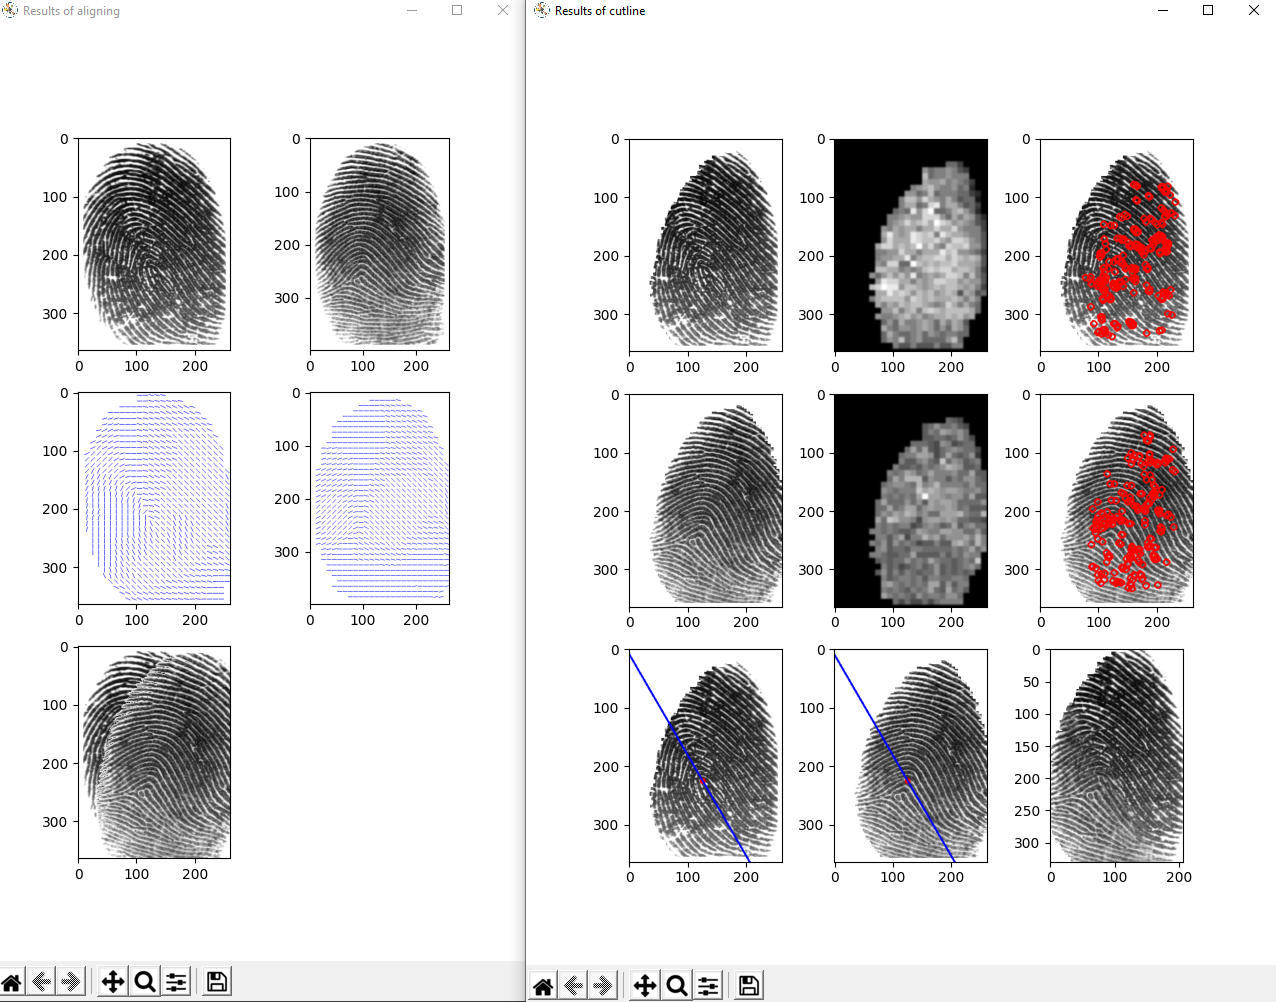
\includegraphics[width=1\linewidth]{obrazky-figures/app_plot.png}}\\
        \caption{Demonstration of plotting the output with steps from morphing application (left window: 1st line = fingerprints with cropped background, 2nd line = orientation fields, 3rd line aligned fingerprints)(right window: 1st and 2nd line = fingerprint with cropped overlaying part, frequency image, minutiae; 3rd line= cutline on 1st and 2ns fingerprint, last is result)}
        \label{fig:app_plot}
\end{figure}

\section{Innovatrics IDKit PC SDK}
IDKit is a tool for creating applications used for fingerprint identification. The IDKit PC SDK supports a number of image formats (RAW, PNG, BMP, JPEG, JPEG 2000, GIF, WSQ, TIF) and is compatible with a wide range of scanners. The tool has support for working with the database, which can be in SQLite / MySQL / MSSQL / Oracle formats. \cite{idkitsdk} On the one hand, this is a very useful function, but in my solution, when I did not find a function in the documentation for comparing fingerprints, which could work without the database, it is made the implementation a bit more difficult.

Innovatrics IDKit PC SDK is officially supported for Windows 32-bit and 64-bit for version 7 and higher, Linux 32-bit and 64-bit (Red Hat), Centos version 7 and higher. \ Cite {idkitsdk}. The application was implemented for Windows 10 and the source code is also submitted with the project, which can be run in Visual Studio 2019.

\label{fca}
\subsection{Fingerprints compare application} 
The application is implemented in C++ using the Innovatrics IDKit PC SDK. Visual Studio 2019 was used for development. It is possible to start evaluation over only three inputs (fingerprint 1, fingerprint 2, morphed fingerprint from two previous ones) when the morphed fingerprint is evaluated against two inputs, but also evaluation over the whole folder is possible when the output is a .csv file that contains the similarity score accumulator, from which it is then possible to create an FMR curve. 

The output of the application are scores for comparison over just three fingerprints (just one run) for both fingerprints from input in comparison with the morphed one. For the whole folder, only the lower score is stored in the .csv file. To load the file into excel, just simply load data from .csv and set delimiter as coma if it is not set automatically.

To run the application, it is first necessary to generate files for the Visual studio using CMake in the build folder. Then, in the project, set the language to C++ 17 (project entry $ \rightarrow $ Properties $ \rightarrow $ C / C ++ $ \rightarrow $ Language $ \rightarrow $ C ++ Language Standard). Finally, set compare as the running project. The source files are here: evaluation \_ modules/ Compare\_ fingerprint/src, the project for Visual studio here: evaluation \_ modules/Compare\_ fingerprint/build/ compare and executable in the Debug pad.

\subsubsection{Application control}
\texttt{./compare.exe -db \_ -s -f1 \_ -f2 \_ -i1 \_ -i2 \_ -gen \_ -geni \_ -suf \_}
\begin{itemize}
    \item \texttt{-db "databaseString"}: The default value is iengine.db 
    \item \texttt{-s}: Save the result to the database
    \item \texttt{-f1 "finger.bmp"}: First fingerprint image
    \item \texttt{-i1 indexOtisku}: First fingerprint index in the database
    \item \texttt{-f2 "finger2.bmp"}: Second fingerprint image
    \item \texttt{-i2 indexOtisku}: Second fingerprint index in the database
    \item \texttt{-gen genFinger.bmp}: Morphed fingerprint image
    \item \texttt{-geni genIndex}: Index of morphed fingerprint image in the database 
    \item \texttt{-suf suffix}: Suffix of images in folder
\end{itemize}

\label{clasifyApp}
\subsection{Console application for classifying fingerprints}
The application is implemented in C++ with the use of the same tools as the previous application described in section \ref{fca} with the use of functions described in section \ref{API}. The application is used to be run through python script src/scripts/divideToClasses.py. That is why the application is having the width and height of the image as arguments. The class is returned as a return code and also printed into the terminal. Return values are integer numbers (0 = unknown, 1 = left loop, 2 = right loop, 3 = arch, 4 = whorl). The lowest size for image on input is 90px width and 90px height.

\subsubsection{Application control}
\texttt{./class\_detect.exe image\_name width height}
\begin{itemize}
    \item \texttt{imagename}: path/to/image.bmp of the fingerprint, which we need to get type of class from
    \item \texttt{width}: Width of fingerprint image
    \item \texttt{height}: Height of fingerprint image
\end{itemize}

\label{classscript}
\subsubsection{Python script}
Python script was created to run application made in C++ over whole folder. Script just recursively goes through folder finds all images, each image puts on input of C++ application and based on returned result copies result into suitable folder. The output folders are arch, left\_loop, right\_loop, whorl and unknown representing each class. 

\textbf{Script control}\\
\texttt{ python divideToClasses.py input\_folder input\_image\_suffix output\_folder \\ path\_to\_class\_detect.exe}
\begin{itemize}
	\item \texttt{input\_folder}: Folder containing fingerprint images
	\item \texttt{input\_image\_suffix}: Suffix of fingerprint images (.bmp/.tiff/...)
	\item \texttt{output\_folder}: Folder for outputting results
	\item \texttt{path\_to\_class\_detect.exe}: path to executable file of application for classifying fingerprints
\end{itemize}

\label{API}
\subsection{Used API description}
This section is describing functions called from C++ API, that were needed for the implementation of fingerprint compare application. The documentation that comes with IDKit is only described how to compare fingerprints with the database. Therefore the database functions are described as well. Most of the functions are returning return values (\texttt{IDKIT\_API}), which can be found in documentation (\cite{idkitsdk}). This work is not describing any of the return values.

\subsubsection{Initialization and Database connect}
Before using whole API first the library has to be initialized, which comes also with license check. This all is made with function \texttt{IDKIT\_API int IEngine\_InitModule()}. Function takes no parameters as same as function that should be called on the of use of the API \texttt{IDKIT\_API int IEngine\_TerminateModule()}. 

For connecting to database that is containing or will contain biometric data \texttt{IDKIT\_API int IEngine\_Connect(const char * connectionString)} function is used. The function takes one parameter and it is a connection string. It is allowed to connect to an SQLite database or memory database. If the string contains only the file name (for example \texttt{idkit.db}) the SQLite connection is selected automatically and if the file does not exist a new one is created. After finishing the job with our database, connections should be closed with the function \texttt{IDKIT\_API int IEngine\_CloseConnection(IENGINE\_CONNECTION con\-nection)}, which takes no parameters.

\subsubsection{Register fingerprint}
The first step in registering a fingerprint is the initialization of the user, which is made by calling API function \texttt{IDKIT\_API IENGINE\_USER IEngine\_InitUser()}. This function returns an ID of the user or NULL in an unsuccessful case. The user is just created and it needs to be said that it is still not registered in the database. To free user function \texttt{IDKIT\_API int IEngine\_FreeUser(IENGINE\_USER user)} is used.

Then we need to load the fingerprint picture and add it to the created user with function \\
\texttt{IDKIT\_API int IEngine\_AddFingerprintFromFile(IENGINE\_USER user,\\ IENGINE\_FINGER\_POSITION fingerPosition, const char * filename)}. The first parameter is the user we just created, the second is the finger to which the image of fingerprint belongs (for more see \cite{idkitsdk} page 106) and last is the filename of the image we are trying to upload.

Now after assigning fingerprint to the user we need to register the user to the database simply by calling \texttt{IDKIT\_API int IEngine\_RegisterUser(const IENGINE\_USER user, int *\\ userID)}, where the first parameter is the user we created and a second is the return value for an ID of a just registered user. To remove user from the database function \texttt{IDKIT\_API int IEngine\_Remove User(int userID)} is used.

To be able to create another user with its own data, the structure of the user needs to be cleared after storing it in the database. This is made by calling the function \texttt{IDKIT\_API int IEngine\_ClearUser(IENGINE\_USER user)}.

\subsubsection{Match fingerprints}
First, we need to prepare the user to be matched like described in the section before or select user from the database with function \texttt{IDKIT\_API int IEngine\_GetUser(IENGINE\_USER user, int userID)}, where the user is output for founded user in the database by userID. The second threshold needs to be set as a deciding parameter with function \texttt{IDKIT\_API int IEngine\_SetParame\-ter (IENGINE\_CONFIG parameter, int value)}. The first parameter is the parameter we want to set (in our case \texttt{CFG\_ SIMILARITY\_THRESHOLD}), and we want to set the value as 0 in our case because we want all the results. Otherwise, all results below the threshold are set to 0. The default value for the threshold is 40.

Matching of two fingerprints is then done with a function \texttt{IDKIT\_API int IEngine\_Match Fingerprint(const IENGINE\_USER user, int fingerprintIndex, int userID, int * bestIndex, int * score)}. The first parameter user is the input user with which the comparison will be made. Parameter fingerprintIndex is an index of the fingerprint that we are comparing. In my implementation, all fingerprints are always saved on index 0. Parameter userId is the id of the user in the database, against which we want to compare our user. Parameter bestIndex is output for best-matched fingerprint index from the user in DB. If this is not important and we do not need this output, the value can be set to NULL and this output is ignored. The last parameter score is the return value of the match score of two fingerprints. If the score falls below the threshold, then the return value is 0.  
  
\label{ffdb}
\subsubsection{Fingerprint image from Database}
To get fingerprint from db function \texttt{IDKIT\_API int IEngine\_GetFingerprintImage(const IENGINE\_USER user, int fingerprintIndex,
IENGINE\_IMAGE\_FORMAT format, unsign\-ed char * fingerprintImage, int * length)} is used. user is an input parameter for the user from which we want to get the fingerprint image, fingerprintIndex is an index of the fingerprint we want to get an image from. Formats are listed in \cite{idkitsdk} on page 106. fingerprintImage is the output image of our fingerprint and length is the size of allocated memory for the resulting image.

\subsubsection{Detect fingerprint class}
To detect the fingerprint class function \texttt{IDKIT\_API int IEngine\_GetFingerprintClass( const unsigned char* fingerprintImage, int
length, int * fingerprintClass)} can be used. Parameters fingerprintImage and length are the same as described in section \ref{ffdb}. Parameter fingerprintClass is output for the class of fingerprint. API supports 4+1 kinds of classes and these are left loop, right loop, arch, whorl + unknown.  

\section{Neurotec Biometric SDK}
Neurotec Biometric SDK is a toolkit for all SDKs (MegaMatcher SDK, VeriFinger SDK, VeriLook SDK, VeriEye SDK, VeriSpeak SDK) from Neurotechnology. It contains all the necessary libraries, documentation and tutorial, and some sample programs. Where, of course, there is the possibility of connecting Different SDKs into one solution. \cite{veri6}

VeriFinger is then only a fingerprint identification tool. VeriFinger allows both 1 to 1 and 1 to N fingerprint comparisons. The Neurotec fingerprint engine has been recognized by NIST in accordance with the MINEX tests. \cite{veri6}

\subsection{Fingerprint match console app}
The application was created according to the tutorial supplied with the Neurotec package in the C language. The application is used to compare fingerprints 1: 1 and returns the similarity score both on the return code of the application and on the standard output. Upload the evaluation folder to start the application \_modules/Neurotec\_Biometric\_6\_0\_SDK\_Tri\-al/src to folder tools Neurotec\_Biometric\_6\_0\_SDK\_Trial and in the project, VerifyFinger changes the source file to main.c. Source files for included: evaluation\_modules/Neuro\-tec\_Biometric\_6\_0\_SDK\_Trial/src/Biometrics/C, executable in: /evaluation\_module\-s/Neurotec\_Biometric\_6\_0\_SDK\_Trial/Bin.

\subsubsection{Console app controls}
\texttt{VerifyFinger.exe fingerprint1 fingerprint2}
\begin{itemize}
    \item \texttt{fingerprint1} Path to the first fingerprint
    \item \texttt{fingerprint2} Path to the second fingerprint
\end{itemize}

A script (runtests.py) written in Python 3.7 was created to automatically evaluate the entire folder, which, as with the Innovatrics version, saves the output to a .csv file for subsequent simple evaluation and creation of an FMR graph. The script is called: \texttt{python3 runtests.py "input /folder" "input.files.extension"}.

For evaluation using VeriFinger v6, it is necessary to have images with DPI 500, for which a python script \texttt{changeDPIFolder.py} was created in the scripts folder. The script is executed as: \texttt{python3 changeDPIFolder.py "input / folder" "DPI"}. The results of the converted files to the required DPI are generated in the \texttt{res} folder and the files have \texttt{.tif} extension.

\chapter{Solution evaluation}
To evaluate the application generating fingerprints by morphing a large database of fingerprints is needed. Although the database used in the paper which was a huge inspiration for this thesis is FVC2002 set A, the solution was not tested over this database for two reasons. The first reason is, that the author tells in the paper, that the pictures were selected randomly, which means that although I would have the database I am not able to check my result application against theirs from the randomness. The second reason is that the database comes with a book \cite{maltoni2009handbook} on CD and in the other way is not freely accessible. Therefore the database of fingerprints from the Brno University of Technology borrowed by Ing. Ondřej Kanich Ph.D. was used.

\section{Fingerprint database EBD}
The database was obtained by Security Technology Research and Development which is the Research group at the Faculty of Information Technology, Brno University of Technology. The database was scanned for academic purposes in several projects. Because of this purpose and legal terms in relating to privacy none of the fingerprints is shown in this work. For visual demonstration of how the application is working were used only public images were found by the Google search engine.

The database in version as I got consists of 9450 fingerprints which means, based on the fact that from every person were taken fingerprints from all fingers on both hands, 945 different people. The fingerprints were obtained by different sensors and this all gave more than enough variety for the application testing.

\section{Results}
To evaluate final applications there was needed to make some reduction in database, mainly because of time complexity. On average one fingerprint takes 37 seconds to generate on my working machine described at the beginning of this chapter. The time differs a lot based on used block size. So mentioned time was measured for 10-pixel blocksize, which was chosen based on the best results overall.

To try most of the variability and most possibilities, first, the fingerprints were sort-out based on their classes with the use of script from section \ref{classscript}. Then 2 folders were created in each class folder with excluding the unknown class folder. Folder a) included 10 randomly chosen fingerprints and folder b) included 100 randomly chosen fingerprints. Then the morphing was run over these folders as each fingerprint from folder a) was combined with every fingerprint from folder b). This created 1000 fingerprints from each class.

To generate interclass fingerprints folder combined was created and from the first two classes (left loop and right loop) 3 random fingerprints were selected, then from the other two, only 2 fingerprints were selected. For folder, b) 25 fingerprints from each class were selected, and then the generation was run the same. This generation was run twice, once for generation from the center and secondly from the core (described in section \ref{mainmorph}). That means, that even with this reduction the time taken by generation was over 102 hours.

After generation, the testing has begun with application from section \ref{clasifyApp} over each folder containing results from each class. 

\begin{figure}[H]
    \centering
        {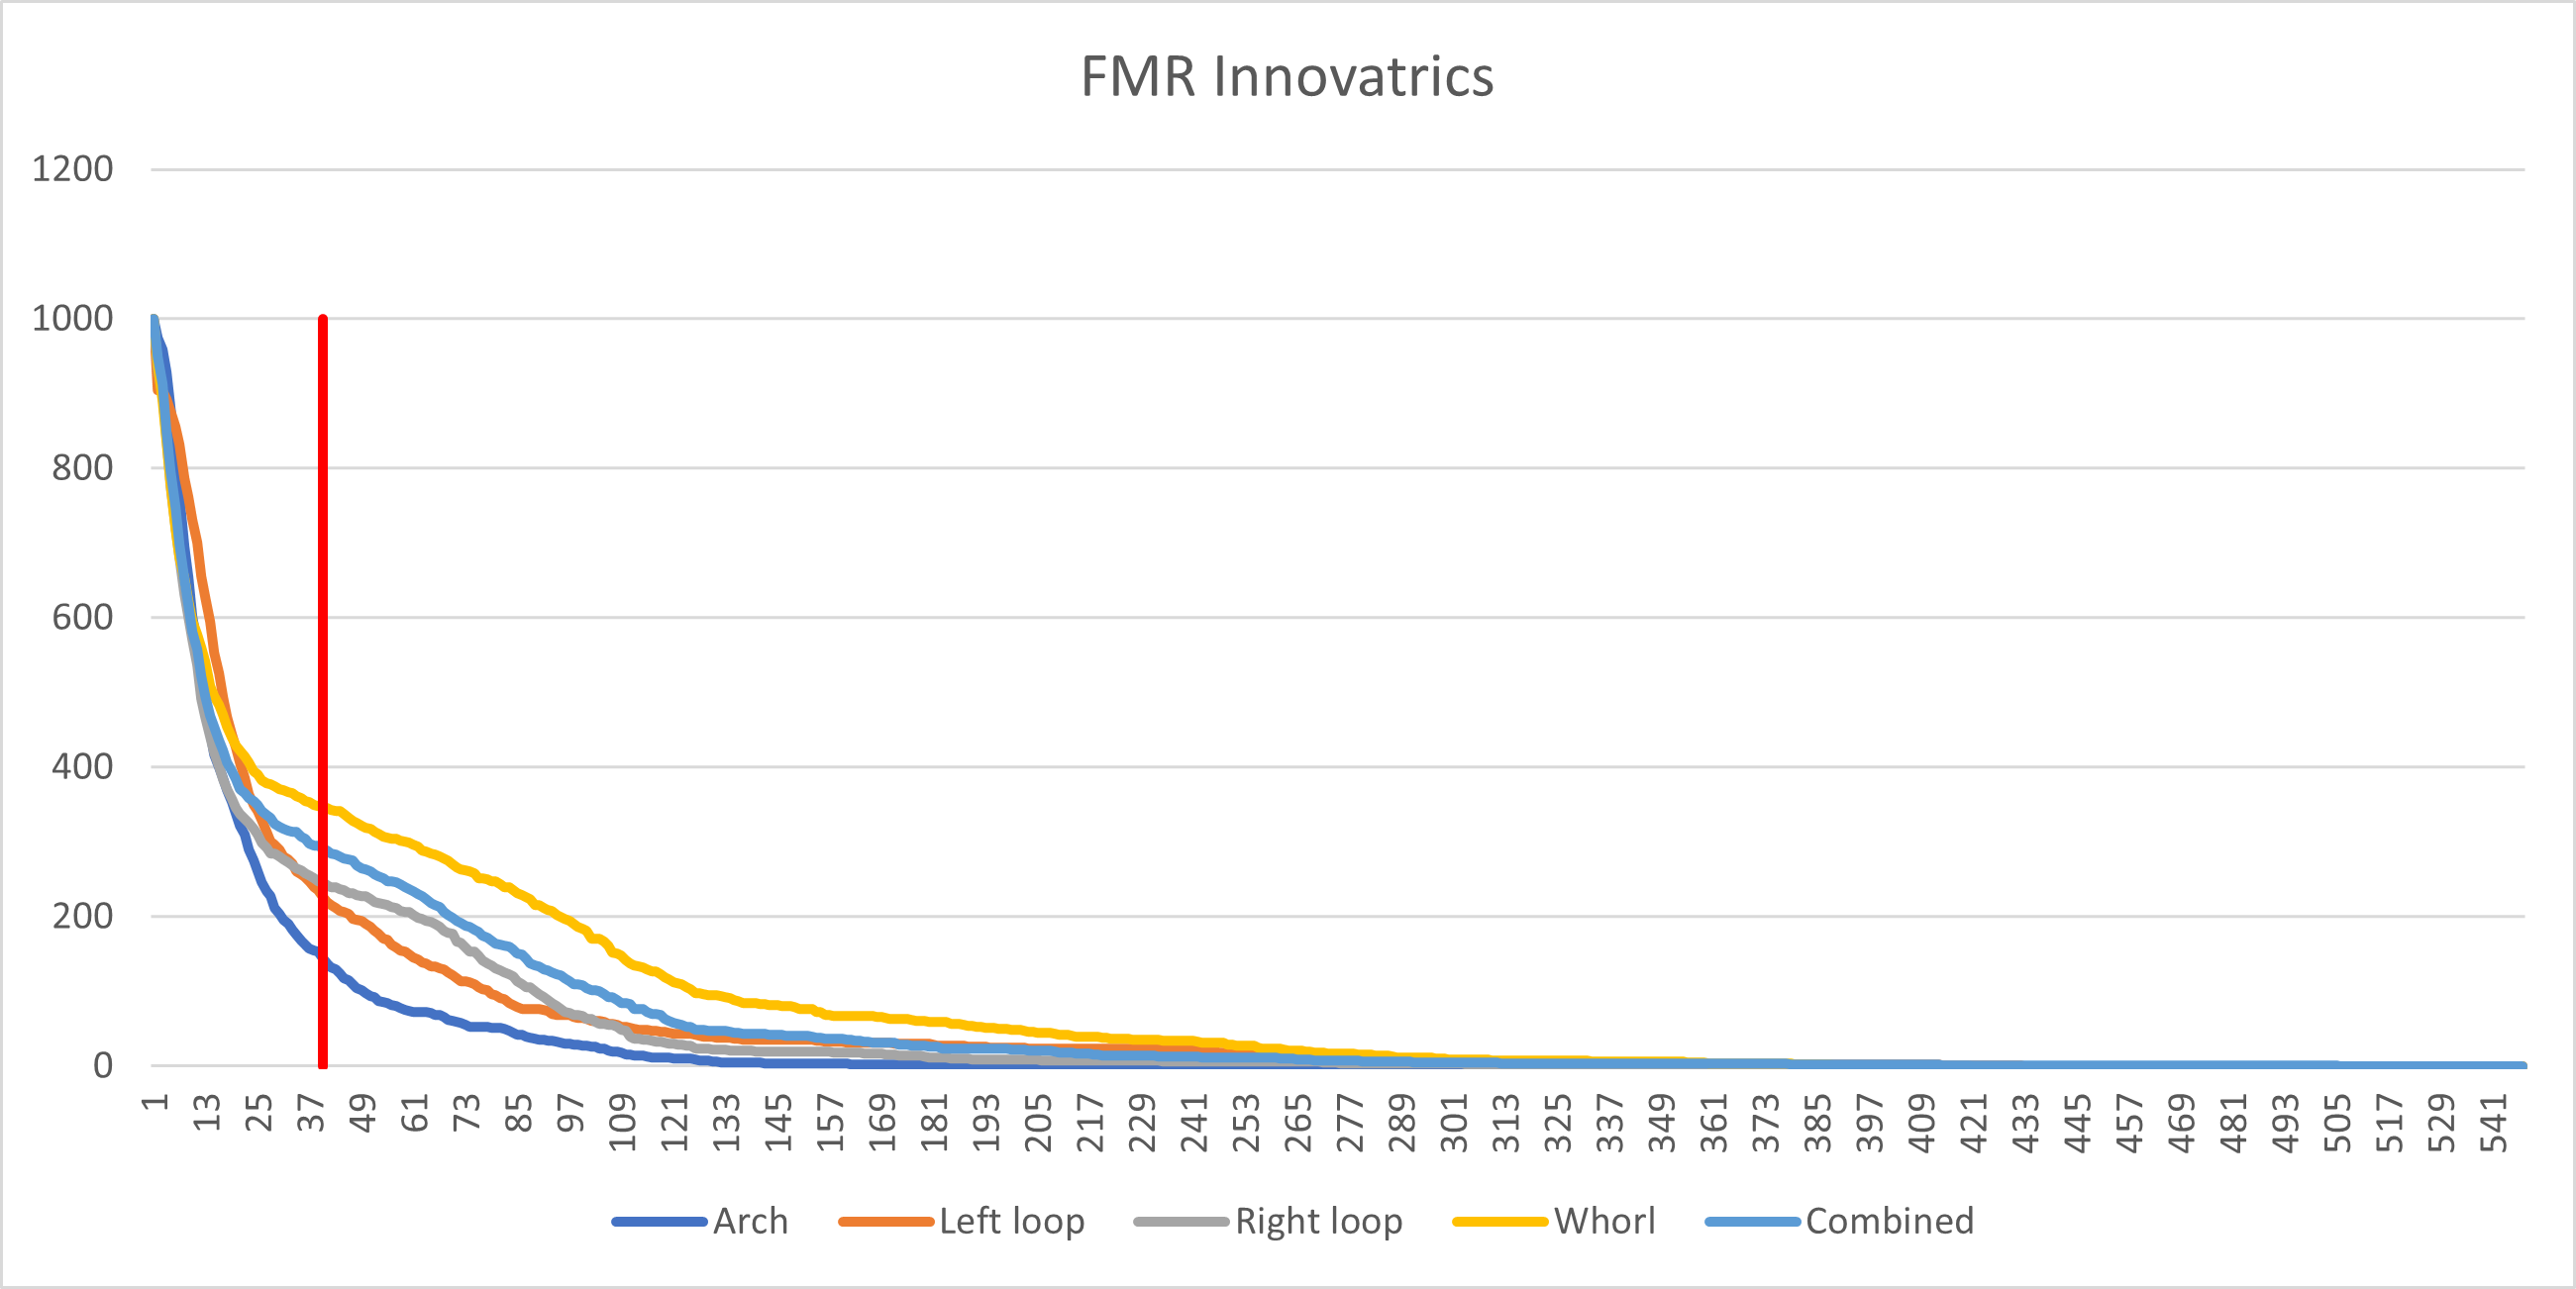
\includegraphics[width=1\linewidth]{obrazky-figures/results_core.png}}\\
        \caption{Results of each class for morphing from section \ref{imageBased1}. Redline is showing default threshold 40.}
        \label{fig:grapf_normal}
\end{figure}

As it can be seen in the first graph \ref{fig:grapf_normal}, the method with morphing fingerprints based on method \ref{imageBased1}, which is using the core of the fingerprint as barycenter is not as effective. With the comparison with the default threshold, only 24.68\% the morphed fingerprints were effective.

On the other side the second method \ref{imageBased2}, which is using center of fingerprint as barycenter for the cutline ended with 41.24 \% with the comparison for default threshold. The results are displayed in the graph \ref{fig:grapf_center}.

\begin{figure}[H]
    \centering
        {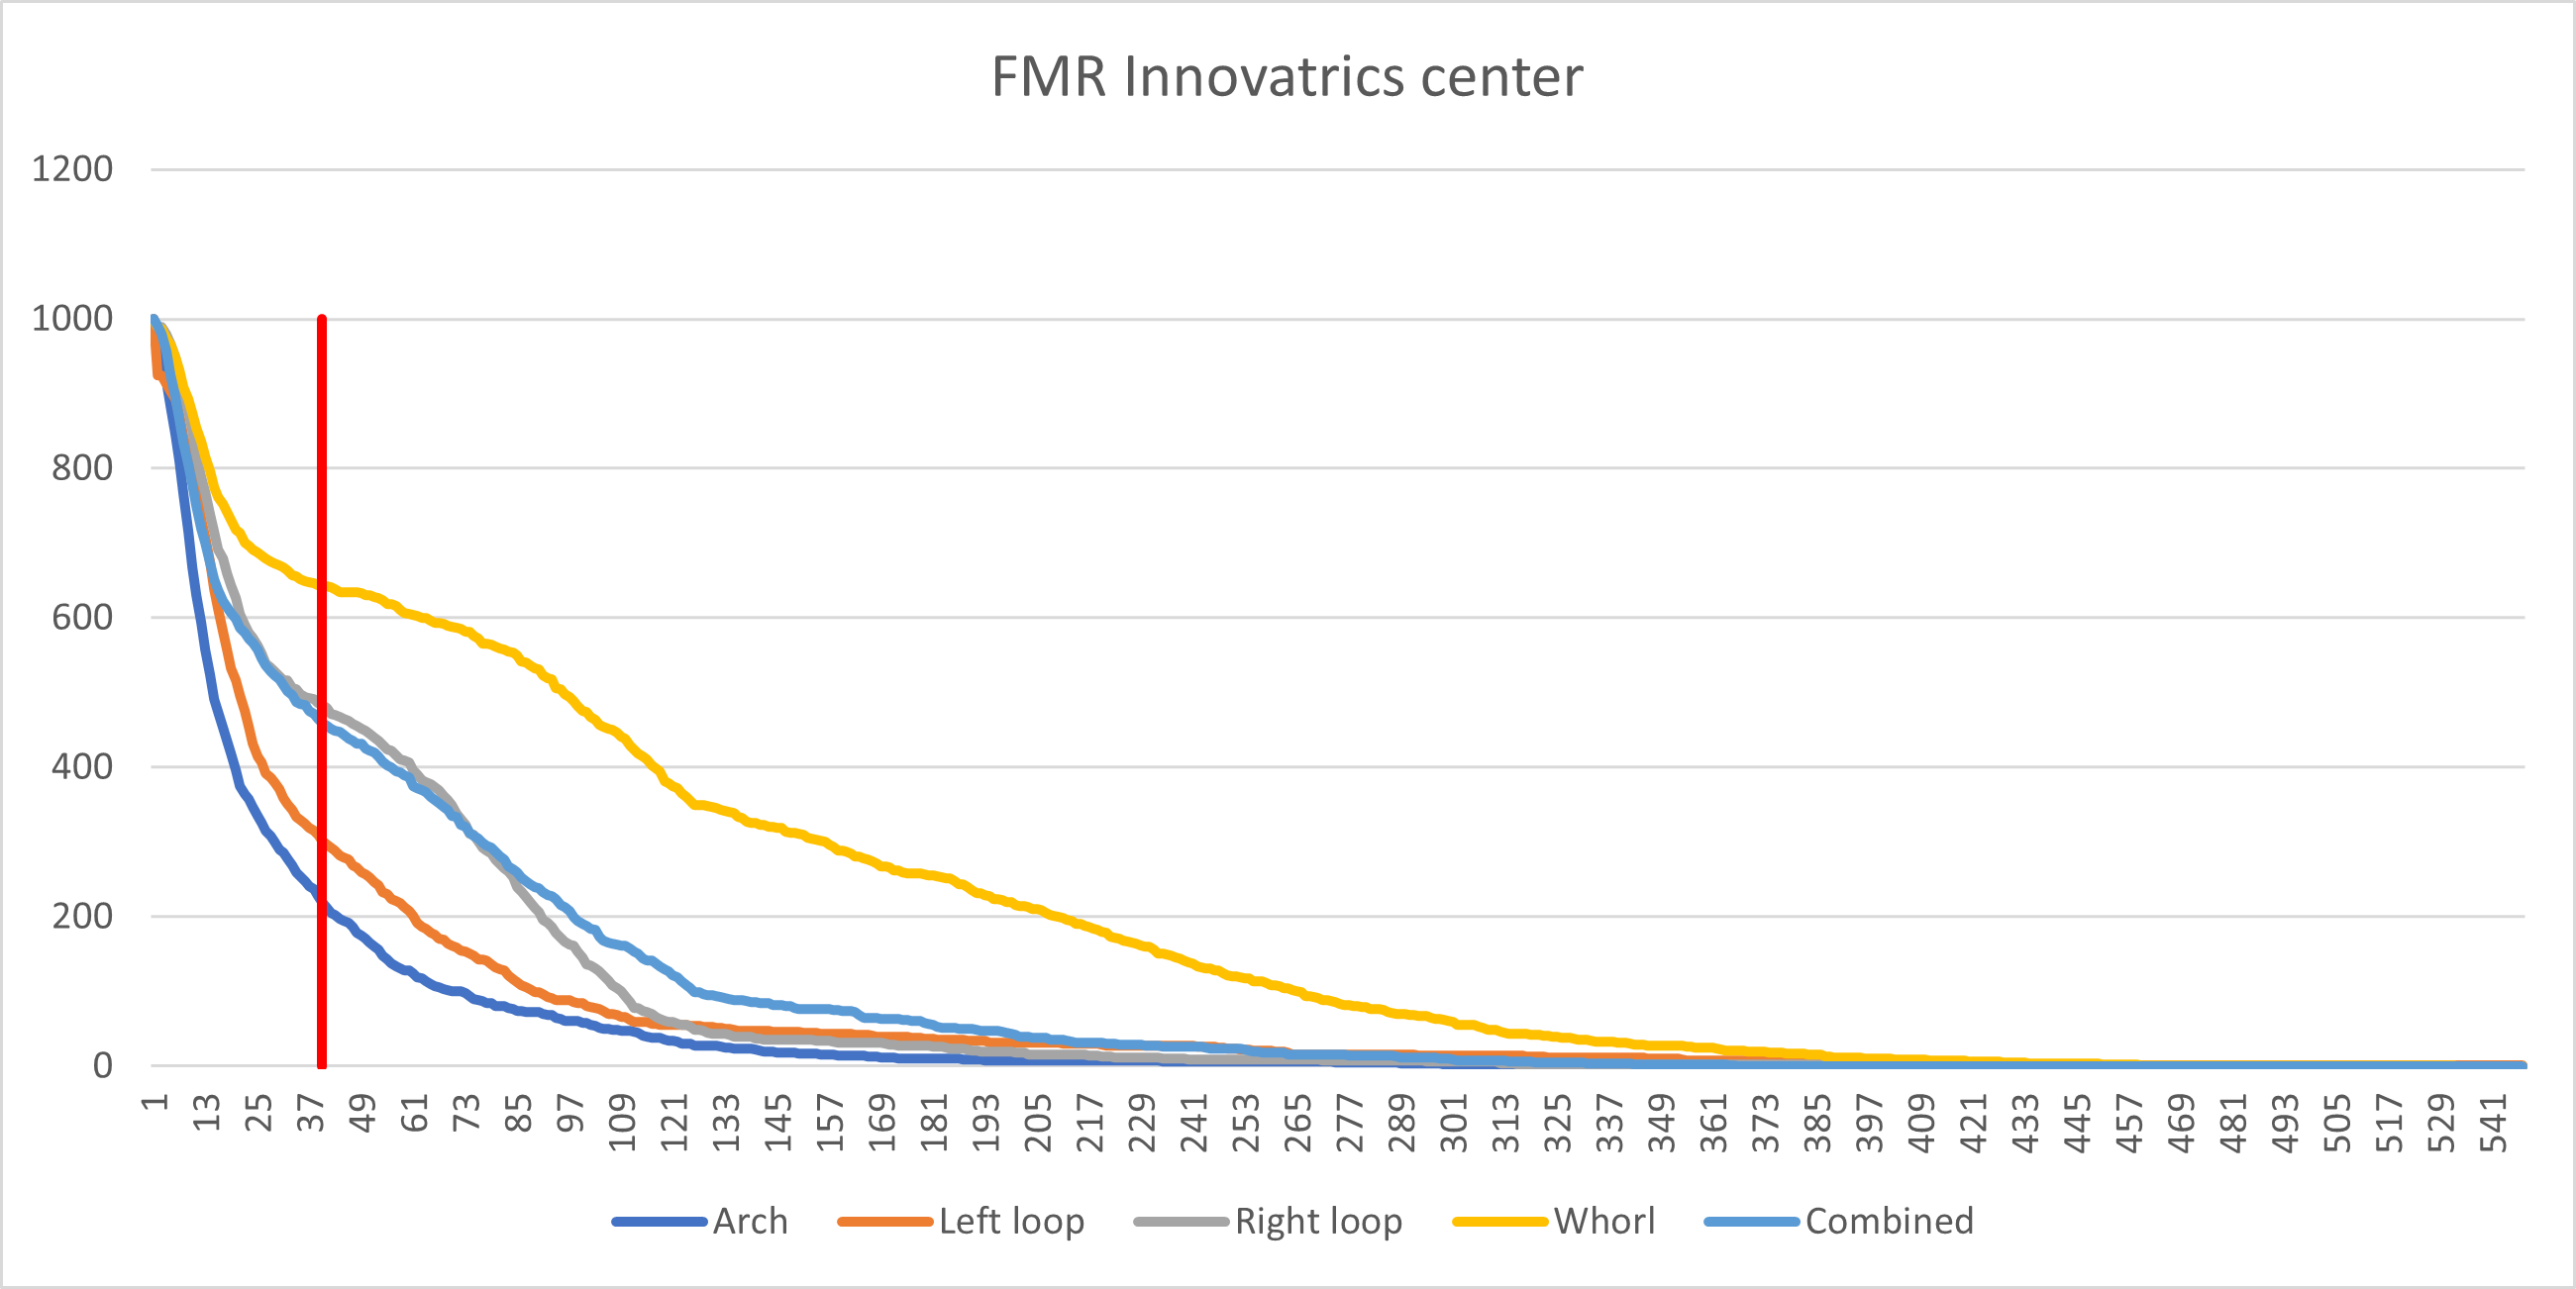
\includegraphics[width=1\linewidth]{obrazky-figures/results_center.png}}\\
        \caption{Results of each class for morphing from section \ref{imageBased2}. Redline is showing default threshold 40.}
        \label{fig:grapf_center}
\end{figure}

\chapter{Conclusion}
This thesis is containing the theory needed for the implementation of the application, but also the theory for capturing fingerprints, which is needed for the testing database. This thesis also covers the design and implementation of application for the generation of fingerprints by the morphing method. The aim of this work was to test these methods against the real biometric systems from companies Innovatrics and Neurotechnology and show the threat which this method is. The first step was research about existing solutions and only two were found in one paper (On the Feasibility of Creating Double-Identity Fingerprints \cite{morphing_paper}). 

The paper contains a description of the two algorithms based on the same technique. Only the image-based morphing was implemented because the second technique was less effective in the author’s results this method was not implemented. It was decided to put more time into improving the image-based morphing and adjust some steps to make the method work better on fingerprints captured in different conditions. Where in the result the improved method was more successful in 16.56 \% than the first one compared to Innovatrics biometric system. The results were generated from a database provided by the Faculty of Information Technology at the Brno University of Technology. 

The finding that not an extremely hard technique for the generation of fingerprints can have a success rate over 41\% against the real system is in my opinion the main benefit of this work. In the future the is a lot of space for improvements. New techniques that are more precise can be found, for example, the cutline can be moved more to the center of minutiae of both fingerprints after the alignment, or trying to make some minimal amount of minutiae from each fingerprint can help maybe to improve the result.

To summarize the whole thesis, starting with chapter 2, the basics about fingerprints and their recognition, capturing the fingerprints and a little bit from mathematical morphology and digital image processing, that is needed to understand are covered there. In chapter 3 the suggested solution for morphing application, starting with pre-processing the input, aligning the fingerprints, computing the cutline, and generating the final result. Chapter 4 then describes the implementation of morphing applications and both applications for detection and description of used Innovatrics API. Chapter 5 then includes measured results and proves that morphed images can be considered a threat to actual biometric systems.
